\documentclass[9pt,twocolumn,twoside]{osajnl}
%% Please use 11pt if submitting to AOP
% \documentclass[11pt,twocolumn,twoside]{osajnl}

\journal{josab} % Choose journal (ao, aop, josaa, josab, ol, optica, pr) 
% OJO: subi solamente el legacy de josab 

% See template introduction for guidance on setting shortarticle option
\setboolean{shortarticle}{false}
% true = letter / tutorial
% false = research / review article
% (depending on journal).

\usepackage{import} %para importar .sty (macros)
\usepackage{labelgraphs} %labelgraphs.sty tiene que estar subido

\usepackage{graphicx}% Include figure files
%\usepackage{subfig}
\usepackage{subcaption}
\usepackage{caption}
\usepackage{float} %para poder usar la H de las figuras

\usepackage[normalem]{ulem}

\newcommand{\ra}[1]{\textcolor{red}{#1}}


%link for edit: https://www.overleaf.com/6147786268rsymdpbhnnnm

%\preprint{APS/123-QED}

\title{Spaser and Optical Amplification Conditions in Graphene-Coated Active Wires}

\author[1]{Leila Prelat} %\email{leilaprelat@gmail.com}
\author[2]{Mauro Cuevas} %\email{mcuevas@austral.edu.ar}
\author[3]{Nicol\'as Passarelli} %\email{n.passarelli2014@gmail.com}
\author[4]{Ra\'ul Bustos Mar\'un} %\email{rbustos@famaf.unc.edu.ar}
\author[1]{Ricardo Depine} %\email{rdep@df.uba.ar}

\affil[1]{Grupo de Electromagnetismo Aplicado, Departamento de F\'isica, Universidad de Buenos Aires and IFIBA, Consejo Nacional de Investigaciones Cient\'ificas y T\'ecnicas,  Ciudad Universitaria, Pabell\'on I, Buenos Aires 1428, Argentina.}

\affil[2]{Consejo Nacional de Investigaciones Cient\'ificas y T\'ecnicas and Facultad de Ingenier\'ia, Universidad Austral, Pilar, Buenos Aires 1629, Argentina.}

\affil[3]{Instituto de Ciencias de Materiales de Barcelona, Consejo Nacional de Investigaciones Cient\'ificas, 08193 Barcelona, Spain.}

\affil[4]{Instituto de F\'isica Enrique Gaviola, Consejo Nacional de Investigaciones Cient\'ificas y T\'ecnicas and Facultad de Ciencias Qu\'imicas, Universidad Nacional de C\'ordoba, Ciudad Universitaria, C\'ordoba 5000, Argentina.}


%\affil[*]{Corresponding author: rdep@df.uba.ar}


\date{Compiled \today}% It is always \today, today,
             %  but any date may be explicitly specified

\begin{abstract}
This work analyzes the optical properties  of a localized surface plasmon (LSP) spaser made of a  dielectric active wire coated with a graphene monolayer. Our theoretical results, obtained by using rigorous electromagnetic methods, illustrate the non-radiative transfer between the active medium and the localized surface plasmons of the graphene. In particular, we focus on the lasing conditions and the tunability of the LSP spaser in two cases: when the wire is made of an infrared/THz transparent dielectric material and when it is made of a metal-like material. 
We analyze the results by comparing them with analytical expressions obtained by us using the quasistatic approximation.
We show that the studied systems present a high tunability of the spaser resonances with the geometrical parameters as well as with the chemical potential of the graphene.
\end{abstract}

%\keywords{Suggested keywords}%Use showkeys class option if keyword
                             %display desired

\setboolean{displaycopyright}{true}

\begin{document}

\maketitle

\section{Introduction}
\label{sec:level1}

%2018 Phys. Rev. B 98, 075411 Absorption sensor based on graphene plasmon quantum amplifier Plasmonics applications are limited by ohmic losses in metal. The use of an active medium has been proposed recently for loss compensation [30,31] and amplification [32] of surface plasmon polaritons (SPPs) propagating along active nanostructures. The mplification can lead to SPP generation [33–37]. Further, it has been understood that a surface plasmon localized at a single nanoparticle can also be coherently generated by nonradiative excitation by an adjacent excited system [38–41]. The experimental realization of such a system, spaser, was reported by several groups [42–46]. In general, the difference between the “SPP generator,” “SPP laser,” and “spaser” is vague, so that they are often  identified [47]. On the other hand, these two devices can be considered as opposed limiting cases, respectively, of a large SPP cavity with quasicontinuous spectra and small (nanoscopic) system with discrete spectra.

Spaser, which stands for surface plasmon amplification by stimulated emission of radiation, is the counterpart of a laser that ideally emits surface plasmons instead of photons. Due to the coupling of localized surface plasmons (LSPs) with the electromagnetic radiation, a spaser can confine light at subwavelength scales, which can be used to provide a controllable source of on-demand high-intensity electromagnetic fields beyond the diffraction limit.
Since its proposal in 2003\cite{BergmanStockman2003} and its first experimental demonstrations in 2009,\cite{noginov2009} a wide variety of geometries and materials/metamaterials for the cavities as well as different compounds for the optical-gain medium have been considered. \cite{Rev1,Rev2,spasergraf1,Rev3,Rev4,Rev5,liu2017,pan2017,pan2018,wang2020,krasnok2020}
%
Since the first experimental demonstrations in 2009, a wide variety of geometries and materials/metamaterials for the cavities as well as different compounds for the optical-gain medium have been considered \cite{BergmanStockman2003,Rev1,Rev2,spasergraf1,Rev3,Rev4,Rev5}.

Despite the development of many advanced spasers, most of the research in this area 
has been focused on natural plasmonic materials such as metals, which have a number of shortcomings, most notably power losses and a fixed charge density which finds applications in the visible and near–infrared range, but not in the mid–infrarred and terahertz (THz) region. 
% un 
However, under adequate circumstances, graphene and other 2D materials also 
%meet the need for surface plasmons 
have the ability to guide surface plasmons while having interesting advantages, such as significantly lower losses and much better tunability. In 2D materials, the constitutive parameters responsible for sustaining plasmon oscillations can be tuned with different techniques, 
%such as 
including chemical doping and field effects. Besides, highly doped graphene shows  lower losses and much longer plasmon lifetimes compared with conventional noble metals, and the spectral range where graphene plasmons can be excited --covering from microwave to optical frequencies-- is significantly wider than the range covered by metallic plasmons. This has implications for a wide range of applications, including environmental management, detection of  biological and chemical agents and non-invasive medical diagnostics. 

%
% Graphene spasers 
%
Motivated by the convenient plasmonic characteristics of graphene and the continuing advances in the fabrication of infrared active optoelectronic materials \cite{infrared1}, a variety of structures with different geometries has been proposed in the literature. For instance, in \cite{spasergraf0} the authors studied the plasmon amplification properties on a plane spaser formed by two dense monolayers of nanocrystal quantum dots deposited onto both sides of a graphene nanoribon. The structure exploits  the spectral tunability via electostatic gating and the high charge carriers mobility in graphene to amplify the low loss surface plasmons in a wide frequency band and with a relatively low threshold.
% low loss surface plasmons
%Regarding to spherical geometry, 
Regarding spherical geometries, in Ref. \cite{spasergraf2} a spaser formed by a graphene nano-sphere wrapped with two-level quantum dots was theoreticaly studied. In particular, the authors evaluate the ability of the system to launch surface plasmons on a flat graphene sheet placed close to the sphere. 
%This system is used to launch surface plasmons on a flat graphene sheet placed close to the sphere. 
In Ref. \cite{spasergraf3} the authors propose a %metal nanoparticles and 
%
graphene--metal %nanodisks 
hybrid plasmonic system surrounded by a quantum dots cascade stack as a nano spaser in the infrared. 
%
In addition, in ref. \cite{ardakani2020} the authors study, within a full quantum approach in the electrostatic regime, a spaser design consisting of a semiconducting cylindrical wire wrapped by graphene and with an active inner core given by a single quantum wire.
Complete literature reviews of the major developments and latest advances in spaser theory, together with a systematic exposition of some of the key results useful to understand the operation of spasers involving both bulk as well as two dimensional plasmonic materials, can be found in Refs. \cite{spasergraf1} (covering up to the year 2016) and \cite{Rev3}. 

%In general, the reader interested in the progress of the spaser theory involving both bulk  as well as two dimensional plasmonic materials is  refer to Ref. \cite{spasergraf1}. 


%Motivated by the convenient plasmonic characteristics of graphene and the continuing advances in the fabrication of infrared active optoelectronic materials \cite{infrared1}, several examples of  graphene-based spasers with different geometries can be found in the literature. For instance, in \cite{spasergraf0} the authors  propose a graphene nanoribon surrounded by  semiconductor quantum dots as a spaser nonosystem. 
%\cite{spasergraf1,spasergraf2,spasergraf3}. Tendria que describir mas lo que se hizo. 

%
% que hacemos
%
This paper 
%deals with the study 
studies the non-radiative transfer of energy from the active medium to LSPs in a not-so-explored configuration where a non-magnetic active medium in the form of a circular wire is coated with a monoatomic layer of graphene that separates the wire from an external, passive dielectric medium. 
%
We consider two different kind of wire cores: nondispersive dielectric, intrinsically nonplasmonic cores, and Drude dispersive, plasmonic cores. In the first case we assume that the core is made of an infrared and THz transparent material. Thus, in this case the graphene layer introduces LSPs 
%localized surface plasmons 
which, otherwise were absent in the bare wire. 
%
In the second case, we assume that the core is made of a metal-like material, such as a semiconductor-based nanocrystal \cite{nanocristal2,nanocristal1,nanocristal4}, capable of supporting LSPs %localized surface plasmons 
for wavelengths between 3 $\mu$m and 10 $\mu$m. Thus, an hybridization between graphene plasmons and those already existing in the bare wire occurs in this case. 
%
%

Based on the resonant behavior of the spaser structure, the LSP characteristics on a graphene cylindrical spaser can be approached in two different but complementary ways. The first one, named the eigenmode approach, involves the  study of  the solutions to the boundary value problem without external sources \cite{CRD},  while the second one, the scattering approach, involves the  study of the electromagnetic response of the structure when it is excited by an external source \cite{maximo1}. The first approach provides the dispersive characteristics of LSPs supported by the structure, such as dispersion curves and damping rates, and the second approach is related to the electromagnetic response %through 
via quantification of scattering observables 
%the scattering and absorption cross sections of the structure 
when LSPs are externally excited. %LSPs dispersion effects are essentially caused by two mechanisms, the geometric details such as the radius of the cylinder and the material dispersion, since graphene behaves as an 2D electron gas with a frequency–dependent conductivity described by the Kubo model \cite{kubo1}. 
%

In a first stage, we use the eigenmode approach \cite{CRD}, particularly well-suited for finding the critical gain values $[\text{Im}\,\varepsilon_1 ]_c$ 
%${\rm Im \mit} \,\varepsilon_1$ 
of the imaginary part of the permittivity of the active medium where the spaser condition is fulfilled.  In the context of the eigenmode approach, these critical gain values can be rigorously obtained by requiring simply that the imaginary part of a modal frequency be zero \cite{smotrova2011,nosich,passarelli2019}. To do so, we use fully retarded methods in all the examples here presented. Besides, we also invoke the quasistatic approximation, valid in the long  wavelength limit, which allows us to obtain analytical expressions that explain the main results obtained with the rigorous theory. 

In a second stage, we use the scattering approach which provides a complementary understanding of plasmonic losses compensation and lasing conditions in terms of scattering observables such as scattering, extinction and absorption cross sections.  

%By using the eigenmode approach, setting the imaginary part of the modal frequencies to zero \cite{nosich,passarelli}, we find critical gain values for ${\rm Im \mit} \,\varepsilon_1$, \textit{i.e.},  the imaginary part of the permittivity of the active medium for which the spaser condition is reached. The fully retarded approach  used to calculate the magnitudes of interest  in all the examples here presented and, \textcolor{forestgreen}{also}, we derive the quasistatic approximation, valid in the long  wavelength limit, which allow us to obtain analytical expressions that explain the main results obtained with the rigorous theory. 
%
% Organization
%

This paper is organized as follows. In section 2 we present a brief description of the electromagnetic  theory based on separation of variables to obtain both the dispersion equation and the electromagnetic fields associated to LSPs supported  by the structure, and we develop the quasistatic approximation. In section 3  we present numerical examples for  dielectric and metal-like wires covered with a graphene sheet. 
Finally, concluding remarks are provided in Section 4. 
%
The system of units used is Gaussian and the $\exp(-i\omega t)$ time--dependence is implicit throughout the paper, 
%represented by the factor , 
with $\omega$ the angular frequency, $t$ the time, and $i=\sqrt{-1}$. The symbols {\rm Re \mit} and {\rm Im \mit} are used for denoting the real and imaginary parts of a complex quantity respectively. 

%Maier ver onenote
%If not using Bib\TeX, you will have to create the \verb+thebibiliography+ environment  and its \verb+\bibitem+ commands by hand.

\begin{figure}[htbp]
    \centering
    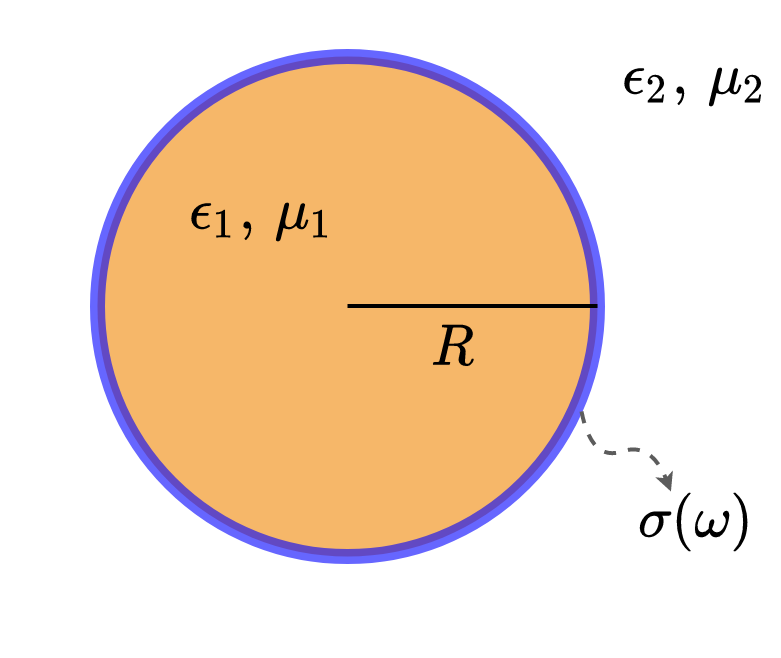
\includegraphics[width=0.35\textwidth]{Leila1Figura1.png}
    \caption{A cylindrical spaser consisting of an active wire coated with a graphene monolayer inmersed in an optically transparent medium.}
    \label{dibujo}
\end{figure}


\section{Theory}
\label{sec:theory}

We consider a graphene--coated cylinder with circular cross--section (radius $R$) centered at $x$=0, $y$=0 (see Fig. \ref{dibujo}) embedded in a transparent medium with real valued electric permittivity $\varepsilon_{2}$ and magnetic permeability $\mu_{2}$. 
%core may be dielectric or conducting 
The active core is assumed to have a magnetic permeability $\mu_{1}=1 $ and a complex valued electric permittivity 
$\varepsilon_{1}={\rm Re \mit} \,\varepsilon_1+ i\,{\rm Im \mit} \,\varepsilon_1$, with ${\rm Re \mit} \,\varepsilon_1>0$ and ${\rm Im \mit} \,\varepsilon_1<0$. Under these conditions the gain coefficient of the core is $\beta_g=-k_0 \,{\rm Im \mit} \,\varepsilon_1/\sqrt{{\rm Re \mit} \,\varepsilon_1}$ \cite{maier2006}, where $k_0=\omega/c$ is the free space propagation constant. 
%
The graphene layer is treated as an infinitesimaly thin, local and isotropic two-sided layer with complex valued surface conductivity $\sigma(\omega)$ and we assume that R is large enough, so that the constitutive properties of the graphene coating are the same of those of planar graphene. In this way, we can write 
$\sigma(\omega)=\sigma ^{intra}(\omega) +  \sigma^{inter}(\omega)$, with intraband ($\sigma ^{intra}$) and interband ($\sigma ^{inter}$) transition contributions given by the high frequency expression derived from the Kubo formula (equation (1), Ref. \cite{kubo1}) 
%
%
\begin{equation} \label{intra}
\sigma^{intra}(\omega)= \frac{2i e^2 k_B T}{\pi \hbar^2 (\hbar\omega+i\gamma_c)} \mbox{ln}\left[2 \mbox{cosh}(\mu_c/2 k_B T)\right],
\end{equation}  
%
\begin{eqnarray} \label{inter}
\sigma^{inter}(\omega)= && 
\frac{e^2}{\hbar} \bigg\{   \frac{1}{2}+\frac{1}{\pi}\mbox{arctan}\left[(\hbar\omega-2\mu_c)/2k_BT\right] \nonumber \\
&& -  \frac{i}{2\pi}\mbox{ln}\left[\frac{(\hbar\omega+2\mu_c)^2}{(\hbar\omega-2\mu_c)^2+(2k_BT)^2}\right] \bigg\}, \\ \nonumber 
\end{eqnarray}  
%
%
where $\mu_c$ is the chemical potential (controlled with the help of a gate voltage), $T$ the ambient temperature, $\gamma_c$ the carriers scattering rate, $k_B$ the Boltzmann constant, $\hbar$ the reduced Planck constant and $e$ the elementary charge. 
%Quantum finite-size effect of graphene is also ignored for a larger graphene structures size compared with 20 nm considered in the whole paper %\cite{quantum1} 
For large doping, $\mu_c\ll k_BT$, the intraband contribution (\ref{intra}) dominates and takes the form predicted by the Drude model, whereas the interband contribution (\ref{inter}) dominates for large frequencies $\hbar \omega > \mu_c$ \cite{kubo1,kubo2}. 

\subsection{Rigorous solution}

In order to derive the modal characteristics of the LSPs in the graphene-coated, circular cross-section wire in terms of wire size, constitutive parameters of substrate and ambient media, and the parameters of the graphene surface conductivity, we use an accurate electrodynamic approach which closely follows the approach of the usual Lorenz–Mie solution for geometries where the radial and angular dependences of the fields can be separated. 
%
Thus, the electromagnetic field of LSPs in this case can be represented in terms of cylindrical multipole partial waves characterized by discrete frequencies. 
%
For surface plasmons localized around the cylinder section the problem can be handled in a scalar way since LSPs are only supported in p polarization, that is, when the electric field is parallel to the main section of the wire \cite{maximo1,CRD} and thus can induce in the graphene coating electric currents along the azimuthal direction $\hat \varphi$. 

The magnetic field $\vec H_{n}(\rho,\varphi,t)$ corresponding to the \mbox{$n$-th} LSP mode is written as
\begin{equation} 
\vec H_{n}(\rho,\varphi,t)= F_{n}(\rho,\varphi) \, \exp{(-i\omega_n t)}\,\hat z\,, \label{magnetico}
\end{equation}
where $\omega_n$ is the complex valued modal frequency. Due to carrier relaxation and radiation losses, plasmon oscillations in passive, dissipative media are always damped and thus the relation 
\begin{equation} 
{\rm Im \mit} \;\omega_n < 0 \,, \label{eqn:condomega}
\end{equation}
must be satisfied. Note that this relation holds even when ${\rm Im \mit} \,\varepsilon_1=0$, that is, when the wire interior is a completely transparent dielectric medium. This is due to the
losses given by the emission of radiation which are always
present.
%
% estuve por decir aca  lo de los valores criticos, pero lo dejo para mas adelante y para la intro
%one of the purposes of this paper is to  Using electromagnetically rigorous numerical simulations [9, 10], we find critical gain values for Ime1, the imaginary part of the electrical permeability of the active medium. For these critical values, the contribution of the active medium exactly compensates the intrinsic losses of the graphene plasmons. 
%
To find frequencies $\omega_n$ and field distributions $F_n$ associated with the $n$-th LSP mode, $F_n (\rho,\varphi)$ is expanded as series of  cylindrical harmonics in the internal 
%($\rho < R$, subscript 1) 
and external 
%($\rho > R$, subscript 2) 
regions. 
%
\begin{equation} 
F_{n}(\rho,\varphi)=   
\begin{cases} 
   c_{n}\;J_n(k_1\rho)\,\exp{i n\varphi}  \,, \text{\, $\rho < R$,}         \\
   a_{n}\;H_n^{(1)}(k_2\rho) \,\exp{in\varphi}\,, \text{\, $\rho > R$,}
\end{cases}      \label{Fz12p}
\end{equation}
where $a_{n}$ and $c_{n}$ are complex coefficients, $n=1,\, 2,\, \ldots \,\infty$, $k_{j}=\frac{\omega}{c}\sqrt{\varepsilon_{j}\mu_{j}}$ ($j=1, 2$), $c$ is the speed of light in vacuum, and $J_n$ and $H_n^{(1)}$ are the $n$-th Bessel and Hankel functions of the first kind respectively.  
%
%
Using the boundary conditions at the graphene layer ($\rho = R$) we get a system of two homogeneous equations for the complex coefficients $a_{n}$ and $c_{n}$, and by requiring that the determinant of this system of equations to be null, we obtain the following dispersion relation for the LSP eigenmodes represented by the cylindrical multipole partial wave \eqref{magnetico} 
% is obtained para salir de tanta voz pasiva
\begin{equation}
\mu_2h_n-\mu_1j_n+  i\mu_1\mu_2 \frac{4\pi}{c^2}\sigma  \omega_n R  j_n h_n =0, \label{eq:disp01}
\end{equation}
where $j_n$ and $h_n$ are
\begin{eqnarray}
&& j_n=\frac{J_n'(k_1 R)}{k_1 R \, J_n(k_1 R)} \,\,\,\,\,\,\,\,\,\, h_n=\frac{H_n'^{(1)}(k_2 R)}{k_2 R \, H_n^{(1)}(k_2 R)} 
\end{eqnarray}
%
The prime denotes the first derivative with respect to the argument of the function.
The eigenfrequency value fixes the relation between amplitudes of the inner and outer region ($c_{n}$  and $a_{n}$ respectively). 
Thus, the spatial part of the electromagnetic field for the \mbox{$n$-th} mode can be written as 
%
\begin{equation} 
\vec H_{n}=   
\begin{cases} 
J_n(k_1\rho)\,\exp{i n\varphi} \hat z \,, \text{\, $\rho < R$,}         \\
\frac{{\textstyle k_1\,\varepsilon_2}}{{\textstyle k_2\,\varepsilon_1}}\frac{{\textstyle J_n'(k_1R)}}{{\textstyle H_n'^{(1)}(k_2R)}}\;H_n^{(1)}(k_2\rho) \,\exp{in\varphi}\,\hat z\,, \text{\, $\rho > R$,}
\end{cases}      \label{campoph1}
\end{equation}
%
\begin{equation} 
{\vec E}_n= 
\begin{cases} 
\frac{\textstyle ic k_1}{\textstyle \omega\varepsilon_1}  \Bigl(in \frac{J_n(k_1\rho)}{k_1\rho}\hat{\rho}- J_n'(k_1\rho)\hat{\varphi}\Bigr) \,\exp{i n\varphi} 
\,, \text{\, $\rho < R$,}         \\
\begin{split}
\frac{\textstyle ic k_1}{\textstyle \omega\varepsilon_1} \frac{\textstyle J_n'(k_1R)}{\textstyle H_n'^{(1)}(k_2R)}& \Bigl(in \frac{\textstyle H_n^{(1)}(k_2\rho)}{k_2\rho}\hat{\rho} \,- \\
&\,\,\, H_n'^{(1)}(k_2\rho)\hat{\varphi}\Bigr) \,\exp{i n\varphi} \,, \text{\, $\rho > R$,}
\end{split}
\end{cases}      \label{campope1}
\end{equation}
%
%
 
\subsection{Gain thresholds}
Optically active medium relies on the stimulated emission of radiation, and that depends, in turn, on the population inversion between an excited and a ground state of the active components of the medium, dyes, quantum dots, rare earth elements, etc. The saturation effects occur when the electromagnetic fields are so intense that a complete population inversion can no longer be sustained by the pumping mechanism, whatever it comes from (radiative or not radiative).
%
Including saturation effects basically involves solving self-consistent rate equations which typically consider the population of excited and ground states of the active material, the spatial distribution of electromagnetic fields, spontaneous emission (Purcell-enhanced or not), and the rate of stimulated emission.
As discussed in several references,\cite{arnold2015,passarelli2016} the consequence of not taking into account saturation effects is that fields go to infinity once optical losses are exactly compensated.
This is not a problem in principle if one is only interested in finding lasing conditions and not the intensity of the electromagnetic fields. Indeed, this property can be used for finding gain thresholds as divergences of properties such as the scattering coefficient.\cite{passarelli2016,passarelli2019}
Instead, here we use another strategy, which is to find the critical value of the imaginary part of $\varepsilon_1$ for which the modal eigenfrequency $\omega_n$ is real.\cite{smotrova2011,passarelli2019,nosich}

Despite its limitations, the strategy used in the present work is still useful to correctly predict the mode that will be lasing (or spasing) and the frequency at which this occurs. Moreover, it can help to estimate the minimum gain required to observe an important enhancement of near and far-fields, see for example Refs. \cite{arnold2015,nosich}. The gain-loss compensation condition discussed in our work, also referenced as the gain threshold,\cite{passarelli2019} does not necessarily mean that most emitted photons are the result of stimulated (coherent) emission since, as calculations including saturation show, spontaneous (incoherent) emission can still be very important (especially if Purcell effects are relevant in the system studied). Requiring that most emitted photons come from spontaneous emission is a more strict condition that demands larger gain values than the ones informed here.\cite{khurgin2012,khurgin2021}

The permittivity of the active medium $\varepsilon_1$ is a frequency-dependent property in general. However, when the response of the system is approximately the same for the frequency interval of interest, the wideband approximation can safely be used. This approximation, which implies taken $\varepsilon_1$ simply as a complex number, is useful for a first exploration of the system as it allows one to calculate the optical response of a system independently of the characteristics of the active medium. As shown for example in Ref. \cite{passarelli2019}, under the appropriate conditions, this approximation provides reliable results for the gain thresholds.

\subsection{Quasistatic approximation}

When the size of the cylinder is small compared to the wavelength, $R<<\lambda=2\pi c/\omega$, we can use the quasistatic approximation. 
 Using the small argument asymptotic
expansions for Bessel and Hankel functions, the dispersion equation \ref{eq:disp01} is written as \cite{CRD}, 
%paper complex frequencies 
\begin{equation}
\varepsilon_1+\varepsilon_2=- \frac{4\pi}{\omega}\sigma(\omega) \frac{i}{R}n. \label{eq:disp02}
\end{equation}
Eq. (\ref{eq:disp02}) allows us to obtain analytic expressions for the LSP frequencies of the two cases: the non-dispersive and dispersive interiors. For large doping ($\mu_c >> k_B T$) and relatively low frequencies($\hbar \,\omega<< \mu_c$) the intraband contribution (\ref{intra}) to the surface
conductivity plays the leading role. In this case, complex roots of 
Eq. (\ref{eq:disp02}) admit analytic expressions that can be obtained as follows. 

\subsubsection{Non-dispersive medium}

By substituting the intraband term  (\ref{intra}) into Eq. (\ref{eq:disp02}), an analytical expression for the eigenfrequency for the non dispersive case is obtained:

\begin{equation}
\label{eq:QE non dispersive}
\omega_n = \sqrt{\dfrac{\omega^2_{on}}{\varepsilon_1+\varepsilon_2}-\left(\dfrac{\gamma_c}{2}\right)^2} -i \dfrac{\gamma_c}{2} \approx \dfrac{\omega_{on}}{\sqrt{\varepsilon_1+\varepsilon_2}}-i\dfrac{\gamma_c}{2},
\end{equation}
where $\omega^2_{on} = \dfrac{4e^2\mu_c n }{\hbar^2R}$ is the effective plasma frequency of the graphene coating for the $n$-th mode. By replacing $\varepsilon_1=\Re\,\varepsilon_1+i\Im\,\varepsilon_1$ into Eq. (\ref{eq:QE non dispersive}) and taking into account that $x=\Im\,\varepsilon_1/(\Re\,\varepsilon_1+\varepsilon_2)<<1$, we can expand $\omega_n$ at first order in $x$,  
\begin{equation}
\label{eq:QE non dispersive2}
\omega_n  \approx \dfrac{\omega_{on}}{\sqrt{\Re\,\varepsilon_1+\varepsilon_2}}-i \frac{1}{2} \Big(\gamma_c+\frac{\omega_{on}\,\Im\,\varepsilon_1}{[\Re\,\varepsilon_1+\varepsilon_2]^{3/2}}\Big).
\end{equation}
%
%If we separate the real and imaginary part of the expression before, we can find the Im($\varepsilon_1$) that makes $\omega_n$ real (the critical value). The analytical expression for the real frequency under the QE approximation is: 
%
%\begin{equation}
%\label{eq:omega crit 1 QE non dispersive}
%\omega^2_n = -\dfrac{\gamma^2_c}{4} + \dfrac{\omega_{on} \Big[\omega_{on} + \sqrt{ \omega^2_{on} - %2\gamma^2_c  (\text{Re}(\varepsilon_1) +\varepsilon_2) } \Big]    }{2 (\text{Re}(\varepsilon_1) %+\varepsilon_2)} 
%\end{equation}
%
%%%%%% %%%%%% %%%%%% %%%%%% %%%%%% 
%creo que definir frecuencia critica aca es confuso porque no depende de la ganancia (Ricardo)
%%%%%%%%%%%% %%%%%% %%%%%% %%%%%% 
Note that, within this approximation, the real part of the eigenfrequency does not depend on the imaginary part of $\varepsilon_1$. In addition, from Eq. (\ref{eq:QE non dispersive2}) we see that the critical value of the imaginary part of $\varepsilon_1$ for which the modal eigenfrequency is real is written as,  %The expression for the other parameter, the imaginary part of $\varepsilon_1$, is:
%
\begin{equation}
\label{eq:im epsi1 crit 2 QE non dispersive}
[\text{Im}\,\varepsilon_1 ]_c = -\dfrac{[\Re\,\varepsilon_1+\varepsilon_2]^{3/2}\, \gamma_c}{ \omega_{on}}=-\dfrac{[\Re\,\varepsilon_1+\varepsilon_2]^{3/2}\, \gamma_c \hbar \, R}{\sqrt{4 e^{2}\mu_c \,n } }    
\end{equation}
%

%\begin{equation}
%\label{eq:im epsi1 crit 1 QE non dispersive}
%\text{Im}(\varepsilon_1) = -\dfrac{\omega^2_{on} \omega_n \gamma_c}{(\omega^2_n + \gamma^2_c/4)^2}    
%\end{equation}

%chequeado con python que QE sin perdidas (lossless) da lo mismo que minimizar im(omega/c) del QE

% Las unidades de $\gamma_c$ tienen que ser unidades de frecuencia entonces en el codigo $\gamma_c = \text{hbargamma}/\hbar$. 

%In all the calculations we have used $\gamma_c=0.0001$ eV and $(\hbar\omega_n)^2 >> \gamma^2_c$, so the term $\gamma^2_c$ is negligible and the expression \ref{eq:omega crit 1 QE non dispersive} can be simplified:

%chequeado con python que $\gamma^2_c$ se puede despreciar en el caso no dispersivo

%\begin{equation}
%\label{eq:omega crit 2 QE non dispersive}
%\omega^2_n \approx \dfrac{\omega^2_{on}}{ \text{Re}(\varepsilon_1) +\varepsilon_2}   
%\end{equation}

%Repeating the same argument for $\text{Im}(\varepsilon_1)$:

%\begin{equation}
%\label{eq:im epsi1 crit 2 QE non dispersive}
%\text{Im}(\varepsilon_1) \approx -\dfrac{\omega^2_{on} \gamma_c}{\omega^3_n}    
%\end{equation}

%The analytical expression for the frequency is used in the formula before to obtain the critical value of Im($\varepsilon_1$). The sign of $\text{Im}(\varepsilon_1)$ is consistent with the temporary dependence used: positive for a passive medium and negative for an active medium. We use the term gain parameter to refer to the modulus of this quantity, $|\Im\,\varepsilon_1|$.

\subsubsection{Dispersive medium}

We consider a mix of nanocrystal and a dye (active medium) for the interior medium. For the metal-like behavior of the nanocrystal we used the Drude model:

\begin{equation}
\label{eq drude lorentz}
\varepsilon_{DL}(\omega) = \varepsilon_\infty - \dfrac{\omega^2_p}{\omega^2 + i\gamma_m \omega}    
\end{equation}
where $\varepsilon_\infty$ is the residual high-frequency response of the material, $\omega_p$ the metallic plasma frequency and $\gamma_m$ the optical loss rate of the Drude material. Therefore, the effective homogenized permittivity of the medium inside the cylinder is:

\begin{align}
\label{eq permeabilidad 1 disp}
\varepsilon_1(\omega) = \varepsilon_\infty - \dfrac{\omega^2_p}{\omega^2 + i\gamma_m \omega} + \underbrace{\varepsilon_{dr} + i\varepsilon_{di}}_{\text{dye}} = \nonumber \\
 \varepsilon'_\infty - \dfrac{\omega^2_p}{\omega^2 + i\gamma_m \omega} + i\varepsilon_{di}
\end{align}
where $\varepsilon'_\infty \equiv \varepsilon_\infty + \varepsilon_{dr}$ and $\varepsilon_{dr} + i\varepsilon_{di}$ represents the contribution of the dye to the effective homogenized permittivity. Note that in this mixed model of the active medium, only the dye is taken in a wideband approximation.

Replacing into equation (\ref{eq:disp02}) the expression of $\varepsilon_1$ given by equation (\ref{eq permeabilidad 1 disp}), after expanding in powers of $y=\frac{\varepsilon_{di}}{\varepsilon'_\infty+\varepsilon_2}$, we obtain, 
%The analytical expression for the second case is:
%
%\begin{align}
%%\label{eqn:QE dispersive}
%\omega_n &= \omega_{1n} - i\omega_{2n}, \nonumber 
%\end{align}
%where
\begin{align}
\label{eqn:QE dispersive2}
\omega_{n}= \sqrt{\dfrac{\omega^2_p+\omega^2_{0n}}{\varepsilon'_\infty+\varepsilon_2}}-\dfrac{i}{2} \nonumber\\ %\quad \omega_{2n} = 
\times \Big[ \dfrac{\omega^2_p\gamma_m+\omega^2_{0n}\gamma_c}{(\omega^2_p+\omega^2_{0n})}+  \varepsilon_{di} \dfrac{\sqrt{\omega^2_p+\omega^2_{0n} }}{(\varepsilon'_\infty+\varepsilon_2)^{3/2}} \Big]
\end{align}
%
%For $\Delta_{di} \not = 0$ (active medium) $\omega_{2n} \not = \text{Im}(\omega_n)$.  
%
Similar to the non dispersive case, the real part of the modal eigenfrequencies does not depend on  $\varepsilon_{di}$ within the range of validity of the quasistatic approximation. Moreover, by equating to zero the imaginary part in Eq. (\ref{eqn:QE dispersive2}), we obtain the critical value for $\varepsilon_{di}$,
%
\begin{equation}
\label{eqn: frecuency crit QE dispersive}
[\varepsilon_{di}]_c = - \dfrac{\omega^2_p\gamma_m+\omega^2_{0n}\gamma_c}{(\omega^2_p+\omega^2_{0n})^{3/2}}(\varepsilon'_\infty+\varepsilon_2)^{3/2}
\end{equation}
%
for which the lasing condition for the $n$-th mode is reached. 

%If we separate the real and imaginary part of the expression frequency $\omega_n$, like in the non dispersive case, we can find the Im($\varepsilon_1$) that makes $\omega_n$ real (the critical value). The analytical expression for the real frequency under the QE approximation is: 
%
%\begin{align}
%\label{eqn: frecuency crit QE dispersive}
%& \omega^2_n = - \omega^2_{2n} +\dfrac{\omega^2_p + \omega^2_{0n} }{2(\varepsilon'_\infty + %\varepsilon_2)} + \\
%& +\dfrac{\sqrt{(\omega^2_p + \omega^2_{0n})\Big[\omega^2_p + \omega^2_{0n} - 8 \omega^2_{2n}\cdot %(\varepsilon'_\infty + \varepsilon_2 )\Big]  }}{2(\varepsilon'_\infty + \varepsilon_2)}
%\end{align}

%Note that, again, the frequency does not depend on the imaginary part of $\varepsilon_{ci}$. 


%In all the calculations we have used $T=300^\circ$ K and $\gamma_c=0.1$ meV. 

%omega_p > omega (plasma)

%The critical value of $\varepsilon_1$ in this case is:

%\begin{equation}
%\label{eqn: im epsi1 crit QE dispersive}
%\varepsilon_{ci} = -\dfrac{ 2\omega_n \omega_{2n}(\varepsilon'_\infty+\varepsilon_2)}{( \omega^2_n -  %\omega^2_{2n})} 
%\end{equation}

%chequeado con python que QE sin perdidas (lossless) da lo mismo que minimizar im(omega/c) del QE

%As in the non dispersive case, we obtained a negative electric permeability, corresponding to an active medium, considering the elected temporal dependency $e^{-i\omega t}$. 

\section{Results}

In this section we solve numerically the fully retarded dispersion relation Eq. (\ref{eq:disp01}) to obtain both the complex eigenfrequencies and the gain thresholds for the first four multipolar modes. The calculation of the gain thresholds requires to find the critical values for which the imaginary part of the eigenfrequency is zero, that is, the values which exactly compensate the plasmon losses. 
To do so, we minimize the modulus of equation \eqref{eq:disp01} with respect to two  variables, namely, the real part of the modal frequency and the optical gain. We use the Nelder-Mead optimization algorithm, taking the values provided by the 
%quasi-static a veces estaba con guión y otras veces si guión. Unifiqué. Chequear cuál. 
quasistatic analytical expressions as initial guesses. We have considered that the wire is immersed in vacuum,  $\varepsilon_2=\mu_2=1$, and that the graphene parameters are $\gamma_c=0.1$meV and T=$300$K in all the calculations. 
%
Regarding the values of the constitutive parameters of the interior medium, and taking into account that our main purpose is to demonstrate spaser characteristics --such as gain thresholds and tunability-- of graphene-coated active wires but not to reproduce the exact behavior of a given material, in the non-dispersive case we have chosen values that are representative of Si- or Ge-based transparent dielectric materials, whereas in the dispersive case we have chosen constitutive parameter values that can be attained using semiconductor plasmonic nanocrystals  \cite{nanocristal2,nanocristal1,nanocristal4}.


%Nelder-Mead 

\subsection{Non dispersive medium}

We consider a dielectric wire of radius $R=0.5\mu$m and $\Re\,\varepsilon_1=4.9$.
In Fig. \ref{fig complex poles non disp}, we plotted the numerical solutions of the dispersion relation, \eqref{eq:disp01}, for the dipolar mode and for three different values of chemical potential $\mu_c = [0.3,0.6,0.9]$ eV. The solutions are displayed parametrically in the complex plane $\Re\,\omega/c$ - $\Im\,\omega/c$, with the imaginary part of $\varepsilon_1$ as parameter. The lowest part of the curves in Fig. \ref{fig complex poles non disp} corresponds to a passive medium ($\Im\,\varepsilon_1= 0$). These curves approach the real axis when the value of $\Im\,\varepsilon_1$ approaches the  critical value $[\Im\,\varepsilon_{1}]_c$ for which the lasing condition for the dipolar order is reached. We have verified that the curves cross the real axis when $|\Im\,\varepsilon_1|> |\Im\,\varepsilon_{1}|_c$. 
%
\begin{figure}[H]
\centering
\includegraphics[width=0.48\textwidth]{results_non_disp/complex_poles1.png}
\caption{Parametric curves of the complex poles (dipolar mode) for a cylinder with  \oneNonDisp $\,\,$ and three values of $\mu_c$.} \label{fig complex poles non disp}
\end{figure}
%
%comentarios: en la figura \label{fig complex poles non disp} las leyendas de los ejes me parecen muy chiquitas, aumentaria el tamaño (SIN tocar los labels de las escalas numericas). %
%
%Under the QE approximation, the frequency does not depend on the imaginary part of $\varepsilon_1$, thus the analytical results hold very well with the numerical solution. 
%
%As can be seen from Fig. \ref{fig complex poles non disp}, the real part of the frequency has a very small variation, it is practically constant. Under the QE approximation, the frequency does not depend on the imaginary part of $\varepsilon_1$ (Eq. \eqref{eq:im epsi1 crit 1 QE non dispersive}) thus the small variation mentioned was expected. 
%
%For $\mu_c=  0.3$eV 
%the  trajectory  starts at  frequency $\omega/c= (0.12216779 - i0.0004) \mu$m$^{-1}$ for $\Im\,\varepsilon_1= 0$, and approaches to the real axis as $\Im\,\varepsilon_1$ is  increased,i.e., the  imaginary  part  of  the  eigenfrequency  increases  while  the real part remains almost constant. This last behavior can be understood from the QE expression  (\ref{eq:QE non dispersive2})  for which  the real part of the eigenfrequency does not depend on the   imaginary part of $\varepsilon_1$.  \textcolor{orange}{We have verified that the imaginary part of the eigenfrequency  $\omega/c$ passes from negative to positive values at a critical value $[\Im\,\varepsilon_{1}]_c$ between $\Im\,\varepsilon_1=x.xxx$ and $\Im\,\varepsilon_1=x.xxx$ for which the lasing condition for the dipolar order is reached}. %
The curves in Fig. \ref{fig complex poles non disp} clearly show that, 
for the values of $\Im\,\varepsilon_1$ considered, the real part of the modal frequency remains almost constant. 
This behavior can be understood from the quasistatic expression (\ref{eq:QE non dispersive2}), where the real part of the eigenfrequency does not depend on the   imaginary part of $\varepsilon_1$. 
%
In addition, we observe that the curves move towards higher $\Re\,\omega/c$ values when the value of the chemical potential is increased, a fact that blueshifts the lasing frequency. This behavior is also predicted by the quasistatic expression (\ref{eq:QE non dispersive2}), which shows that $\Re\,\;\omega_n$ behaves like $\sqrt{\mu_c}$.

%The chemical potential $\mu_c$ changes the shape of the solutions, being less curves for bigger chemical potential (more conductive). \textcolor{red}{completar?}

%\subsubsection{Critical values}
%\label{sec critical values nondisp}

Fig. \ref{fig critical values non disp} shows the  critical values  $[\Im\,\varepsilon_{1}]_c$ for which the lasing condition is reached as a function of the chemical potential of graphene for the dipolar mode (Fig. \ref{fig critical values non disp}a) and for quadrupolar, hexapolar and octupolar modes  (Fig. \ref{fig critical values non disp}b).  
%
\begin{figure}[H]
\centering
\includegraphics[width=0.48\textwidth]{results_non_disp/im_epsi1_vs_mu.png}
\caption{Critical values of ${\rm Im \mit} \,\varepsilon_1$ as a function of $\mu_c$ for 
a cylinder with \twoNonDisp. a) The dipolar. b) the quadrupolar, hexapolar and octupolar modes.}
\label{fig critical values non disp}
\end{figure}
%
From these curves 
we see that the critical gain coefficient $\beta_g=-k_0\, \Im\,\varepsilon_1/\Re\,\varepsilon_1$ for which the dipolar mode reaches the gain threshold is greater than that corresponding to the other modes. 
 %in Fig. \ref{fig critical values non disp} 
This is due to the fact that  radiation losses for the dipolar mode are higher than for  other modes (see \cite{CRD} Table 1), a behavior not predicted by the quasistatic approximation (\ref{eq:QE non dispersive}).
 %Also, as indicated by figure \ref{fig critical values non disp}a, the critical value of the dipole mode varies less as the chemical potential varies, compared to the other modes (\textcolor{red}{por que le afecta menos lo mayor o menor conductor al modo dipolar?}). 
%
%
On the other hand, Eq. (\ref{eq:im epsi1 crit 2 QE non dispersive}) anticipates that in the quasistatic approximation, the critical gain parameter behaves like $\mu^{-1/2}$.  We observe that while the numerical curves for the higher (quadrupolar, hexapolar and octupolar) modes in Fig. \ref{fig critical values non disp}b exhibit this behavior, the numerical curve for the dipolar mode in Fig. \ref{fig critical values non disp}a does not.
%
This is in accordance with the fact that the higher the multipole modal frequency $\omega_n$, the better the 
%quasi-static con guión o sin guión, pero siempre igual
quasistatic approximation, 
%holds, 
since the effective wavelength of higher multipoles becomes shorter and the LSP modes perceive the circular graphene sheet as increasingly flat (see Ref. \cite{CRD}, equations (11)-(13)). 

%As mentioned before, the dipolar mode did not behave like $\mu^{-1/2}$, instead the values followed a curve line (Fig. \ref{fig critical values non disp}a)). \textcolor{blue}{The movement of the charges, inside and out the cylinder, is curve and explain the critical values obtained for the dipolar mode}. 


%For all modes, when the chemical potential approaches to zero, the critical value decreases. \textcolor{blue}{That is consistent with the fact that the real part of the permeability is positive thus when $\mu_c=0$ the complex pole disappear and the critical value diverges. }For the higher modes, as $\mu_c$ increases the modulus of the critical value minimizes (Fig \ref{fig critical values non disp}b)). This is consistent with the behavior observed in \cite{CRD} Fig.7: the losses of the graphene, represent by the imaginary part of the frequency, minimizes when the chemical potential increases thus the optical gain needed is smaller. Varying the chemical potential $\mu_c$ is useful to tune damping rates, as seen in \cite{CRD}, consequently, is useful to tune the optical gain. In the dipolar mode, we also observed the mentioned behavior for $\mu_c$ in range [0.3-06]eV (Fig \ref{fig critical values non disp}a)). 

%The modal real frequencies (critical condition) separate when the value of $\mu_c$ increases (not show, \textcolor{red}{mostrarlo omega/c vs mu?}) 

%Leila: 
%\textcolor{blue}{The absolute value of the critical values in the numerical solution are bigger than in the quasi-static approximation because the QE underestimate the losses (not shown)}, no lo pondria a menos que se grafique una curva comparativa. 

%\textcolor{orange}{Ver si queda claro que estamos hablando siempre de calculos numericos}
% $\epsilon_1$ = 3.9 - i3.53072e-02,  y $\omega/c$ = 1.34005e-01 1/$\mu$m
%\subsubsection{Cross-sections}
 
In order to discuss the previous results in terms of scattering observables, 
% we calculated the scattering, absorption and extinction  cross sections.  
in Fig.s \ref{fig Qscat non disp}, \ref{fig Qabs non disp} and  \ref{fig Qext non disp} 
we plot color maps in the $\omega/c$ - $\Im\,\varepsilon_1$ plane of the scattering, extinction and absorption cross sections, respectively. 
%
Fig. \ref{fig cross sections nondisp}a illustrates the enhancement of the scattering efficiency for frequencies  and gain parameters near the values $\omega_c/c=0.134$ and $[\Im\,\varepsilon_{1}]_c = -0.0353072$ for which the lasing condition for the dipolar mode is reached. Near this critical condition, the scattering cross section diverges and the width at half maximum of the resonance tends to zero, 
%according 
in agreement with the fact  that the eigenfrequency tends to be real. 

%the improvement of the cross sections given by adding an active medium with critical value of Im($\varepsilon_1$). The cross sections show an evident dipolar nature even though the first thirty modes have been considered. This dipolar behavior is due to the near fields. 

\begin{figure}[t]
    \centering
    \captionsetup[subfigure]{justification=centering}
    \subfloat[Scattering]{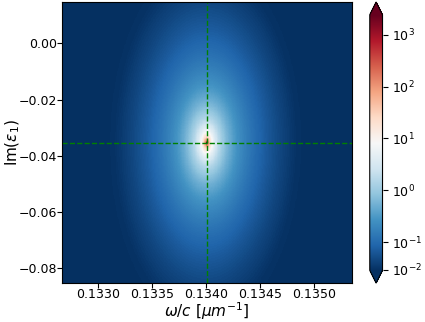
\includegraphics[width=0.22\textwidth]{results_non_disp/Qscat2D_modo1_mu0.3000.png}\label{fig Qscat non disp}}
    \captionsetup[subfigure]{justification=centering}
    \subfloat[Absorption]{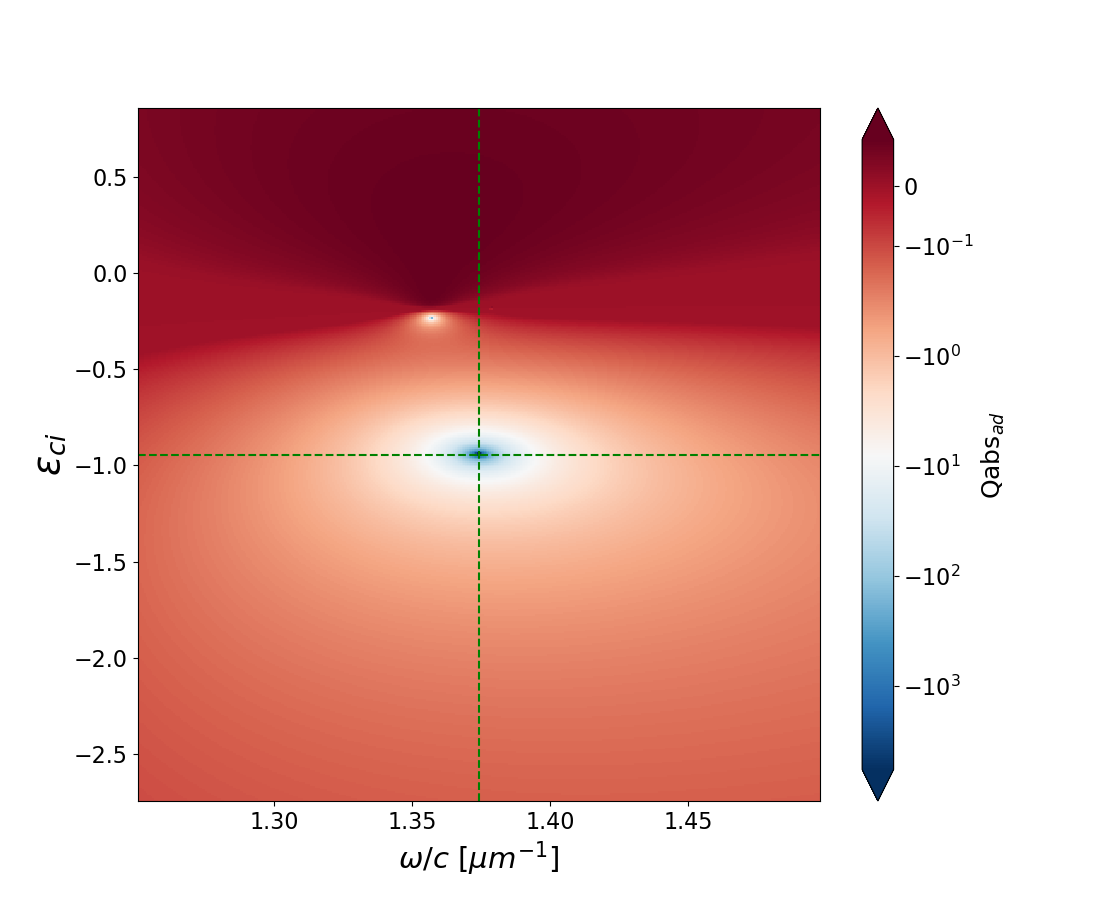
\includegraphics[width=0.22\textwidth]{results_non_disp/Qabs2D_modo1_mu0.3000.png}\label{fig Qabs non disp}}
%    \newline
    \captionsetup[subfigure]{justification=centering}
    \subfloat[Extinction]{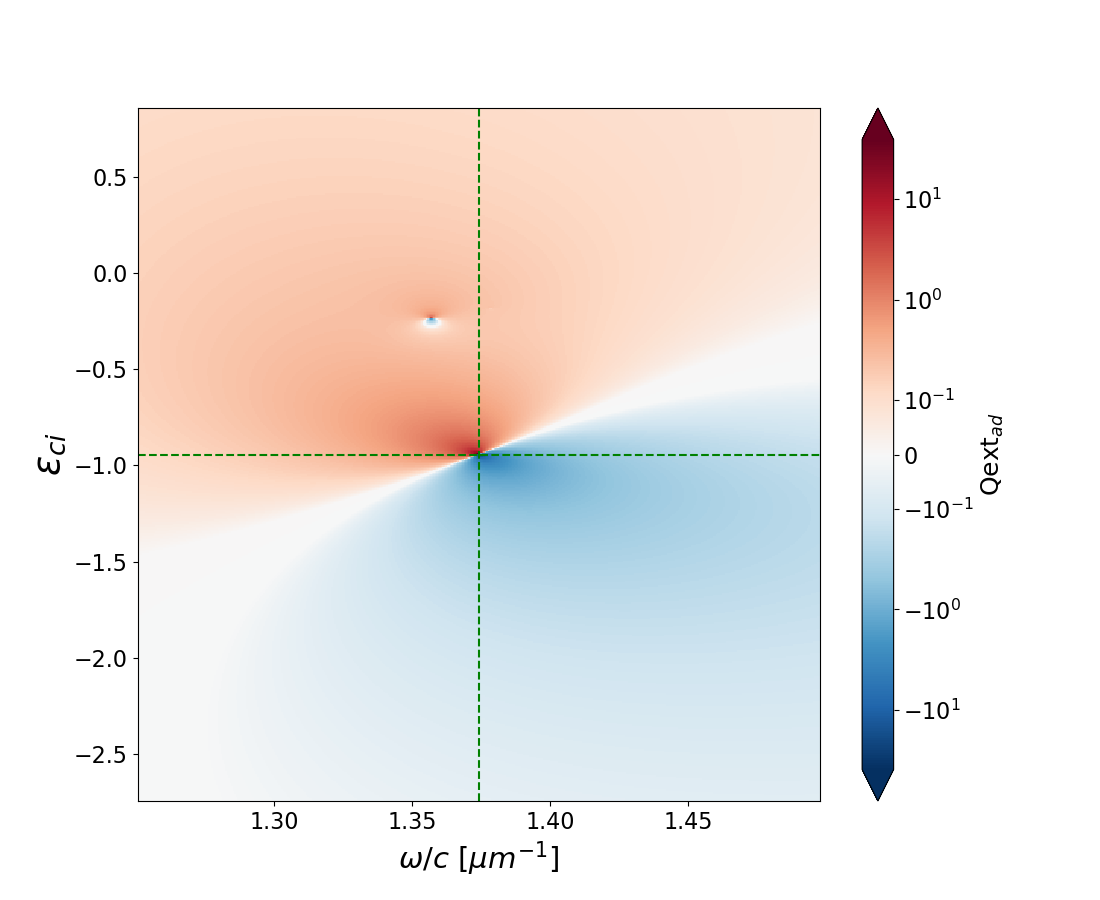
\includegraphics[width=0.22\textwidth]{results_non_disp/Qext2D_modo1_mu0.3000.png}\label{fig Qext non disp}}
    \caption{Cross-section for a cylinder with \threeNonDisp. In green dotted lines: the critical values found before (Fig. \ref{fig critical values non disp})}
    \label{fig cross sections nondisp}
\end{figure}



Fig. \ref{fig Qext non disp} shows two regions separated by a  green  curve  for  which  the  extinction  cross  section  is  equal to zero. Above this curve the extinction cross section is possitive (red  region),  indicating  that  plasmonic  losses  (ohmic  more radiative losses) are not compensated, while below this curve the extinction cross section is negative, indicating  that  plasmonic losses are fully compensated. 
%The critical point $\omega_c/c$ and $[\Im\,\varepsilon_{1}]_c$ falls on the full loss compensation curve, according with the fact that the lasing condition implies the full loss compensation condition \cite{Rev1}. 
The critical point $\omega_c/c$ and $[\Im\,\varepsilon_{1}]_c$ falls on the full loss compensation curve, since the lasing condition implies the full loss compensation condition \cite{Rev1}. 
From Fig. \ref{fig Qabs non disp} we see that the region for which the absorption cross section is positive falls above the full loss compensation curve, indicating that ohmic losses are compensated for an optical gain coefficient value which is lower than that corresponding to the critical value. This is an indication of deviations from the quasistatic approximation, which does not present radiation losses. %,    $\beta_1|<|\Im\,\varepsilon_{1c}|$.  



%\textcolor{blue}{As can be seen from Fig. \ref{fig Qabs non disp}, the optical gain compensates the radiation losses first, when absorption reaches zero}. Then the optical gain compensates exactly all the losses until absorption minimizes (Fig. \ref{fig Qabs non disp}). In the critical condition, the scattering maximizes (Fig. \ref{fig Qscat non disp}) and the extinction reaches zero (Fig. \ref{fig Qext non disp}). The extinction changes sign around the spaser condition \cite{passarelli} and this behavior is illustrated in Fig. \ref{fig Qext non disp}. 

%The local maximum observed in the scattering, the local minimum observed in the absorption and the zero observed in the extinction correspond to a plasmonic resonance and can be obtained from the poles of the coefficients $a_n$ and $c_n$ ($p$ polarization) of the multipole expansions for the electromagnetic field. No enhancements were observe in the cross sections for the $s$ polarization (not shown) which is consistent with the fact that localized surface plasmon are not supported in the $s$ polarization. A necessary condition for the existence of localized surface plasmon in the graphene circular cylinder is that the electric field has to induce electric currents along the azimuthal direction $\hat{\varphi}$. However the electric field can only induce electric currents along the $\hat{z}$ direction thus the localized surface plasmon are not supported in the $s$ polarization. 


%\subsubsection{Fields}

To gain insight about the active medium inclusion on the electromagnetic field scattered by the wire, in Fig. \ref{fig fields nondisp} we plotted the spatial distribution of the magnetic field $H_z$, at the resonance frequency for the first four modes (dipolar, cuadrupolar, hexapolar and octupolar),  near the wire with an active medium ($\Im\,\varepsilon_1 \neq 0$, left column) and without an active medium ($\Im\,\varepsilon_1 = 0$, right column).  The direction of the plane wave incidence is 
%from the left to the right. 
from  left to right.
%
Each modal field has been  normalized with respect to its own maximum field. 

%The magnetic field along the $\hat{z}$ direction for the first four modes (dipolar, cuadrupolar, hexapolar and octupolar) is shown in Fig. \ref{fig fields nondisp}.

\begin{figure}[ht!]
    \centering
    %\subfloat[mode 1 with active medium inside]
    \captionsetup[subfigure]{justification=centering}
    \subfloat[mode 1, $\Im\,\varepsilon_1 \neq 0$]
    {\includegraphics[width=0.2\textwidth]{results_non_disp/modHz_modo1_mu0.3000.png}}
    \hspace{1mm}
    \captionsetup[subfigure]{justification=centering}
    \subfloat[mode 1, $\Im\,\varepsilon_1 = 0$]
    {\includegraphics[width=0.2\textwidth]{results_non_disp/modHz_loss_modo1_mu0.3000.png}} 
    \newline
    \captionsetup[subfigure]{justification=centering}
    \subfloat[mode 2, $\Im\,\varepsilon_1 \neq 0$]
    {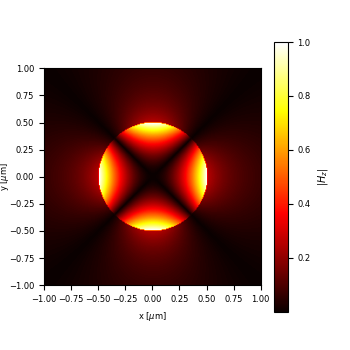
\includegraphics[width=0.2\textwidth]{results_non_disp/modHz_modo2_mu0.3000.png}}
    \hspace{1mm}
    \captionsetup[subfigure]{justification=centering}
    \subfloat[mode 2, $\Im\,\varepsilon_1 = 0$]
    {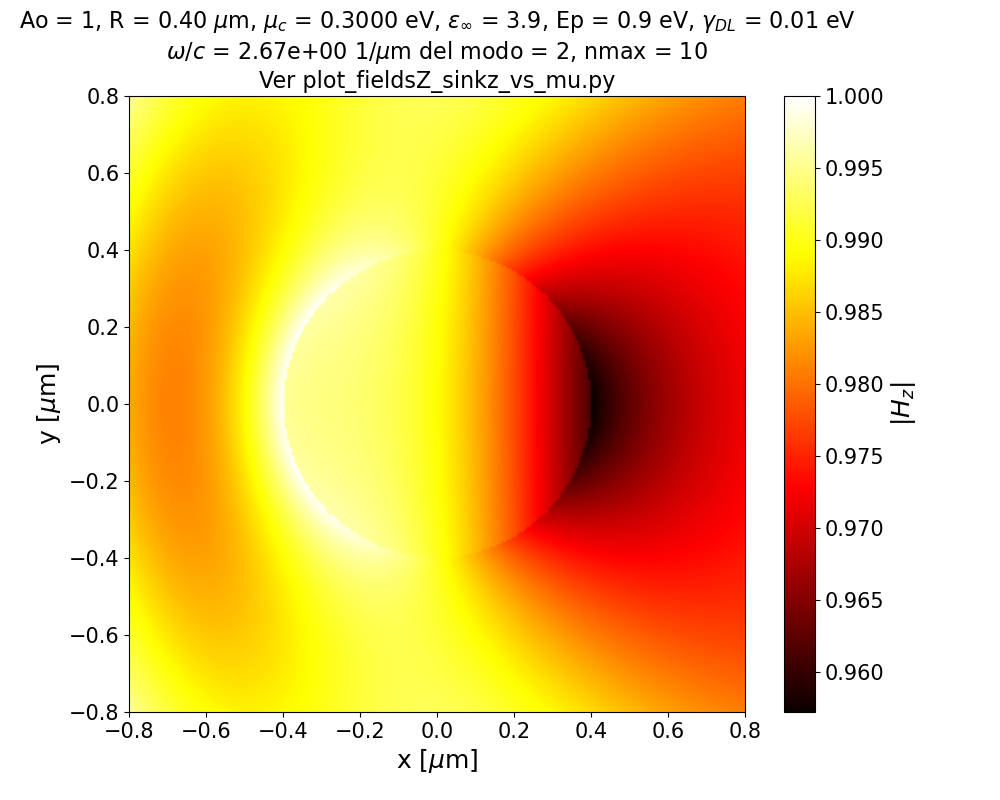
\includegraphics[width=0.2\textwidth]{results_non_disp/modHz_loss_modo2_mu0.3000.png}} 
    \newline
    \captionsetup[subfigure]{justification=centering}
    \subfloat[mode 3, $\Im\,\varepsilon_1 \neq 0$]
    {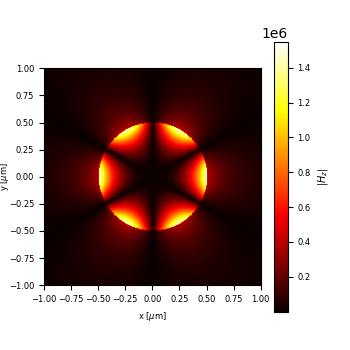
\includegraphics[width=0.2\textwidth]{results_non_disp/modHz_modo3_mu0.3000.png}}
    \hspace{1mm}
    \captionsetup[subfigure]{justification=centering}
    \subfloat[mode 3, $\Im\,\varepsilon_1 = 0$]
    {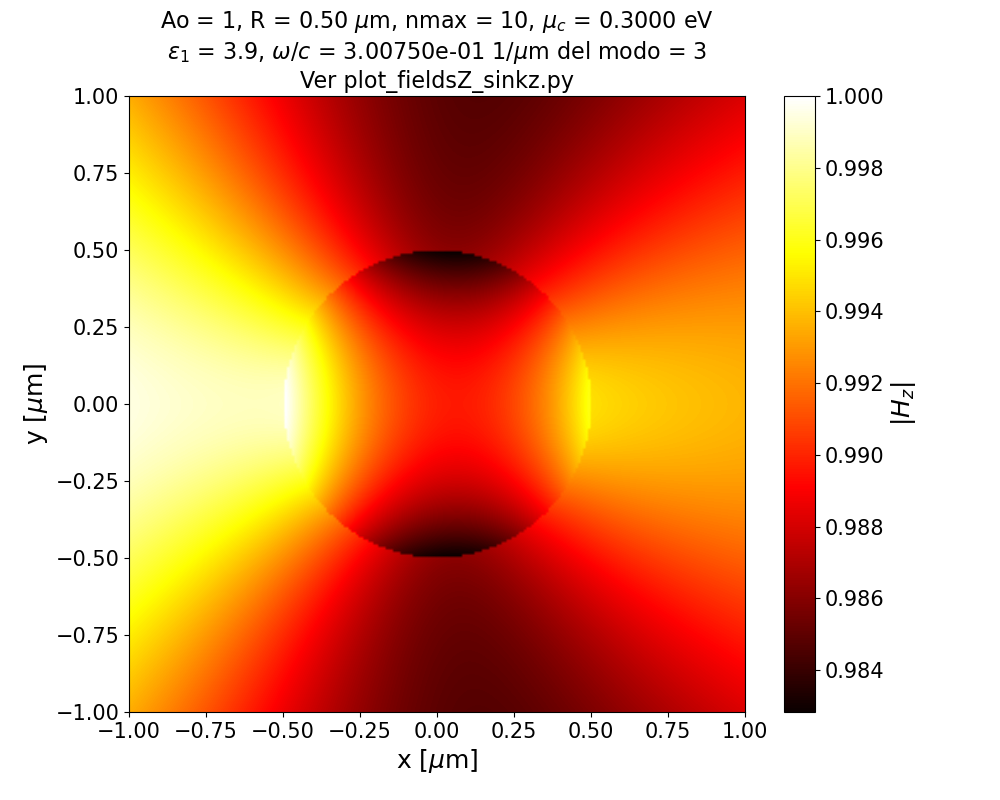
\includegraphics[width=0.2\textwidth]{results_non_disp/modHz_loss_modo3_mu0.3000.png}} 
    \newline
    \captionsetup[subfigure]{justification=centering}
    \subfloat[mode 4, $\Im\,\varepsilon_1 \neq 0$]
    {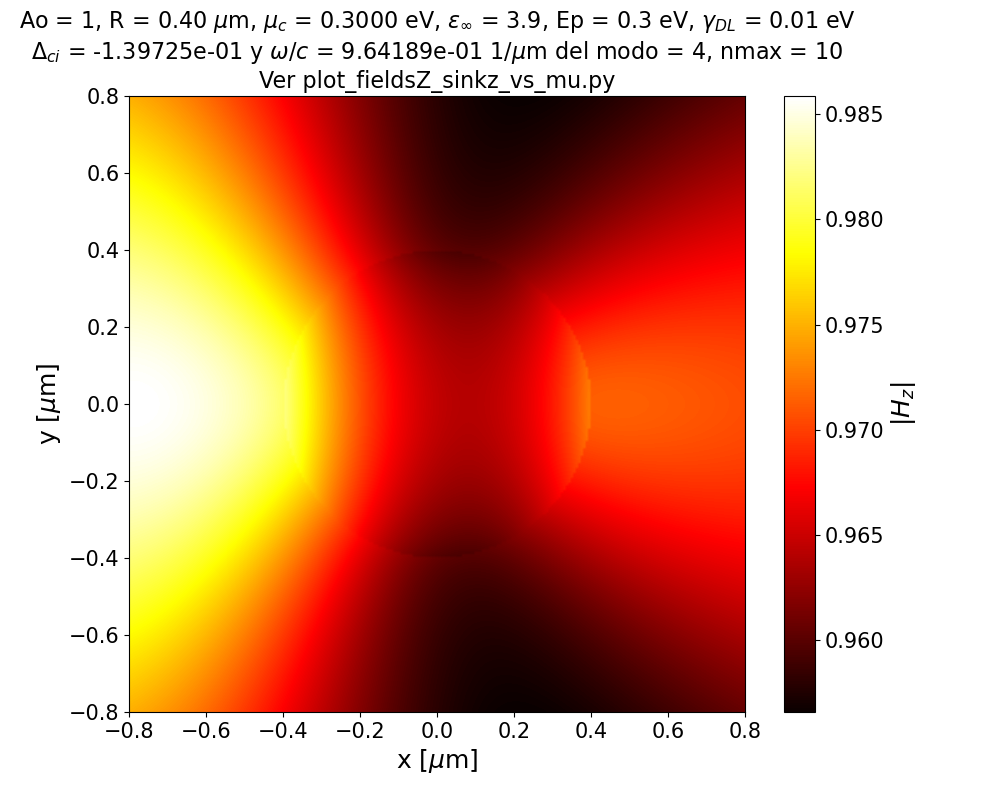
\includegraphics[width=0.2\textwidth]{results_non_disp/modHz_modo4_mu0.3000.png}}
    \hspace{1mm}
    \captionsetup[subfigure]{justification=centering}
    \subfloat[mode 4, $\Im\,\varepsilon_1 = 0$]
    {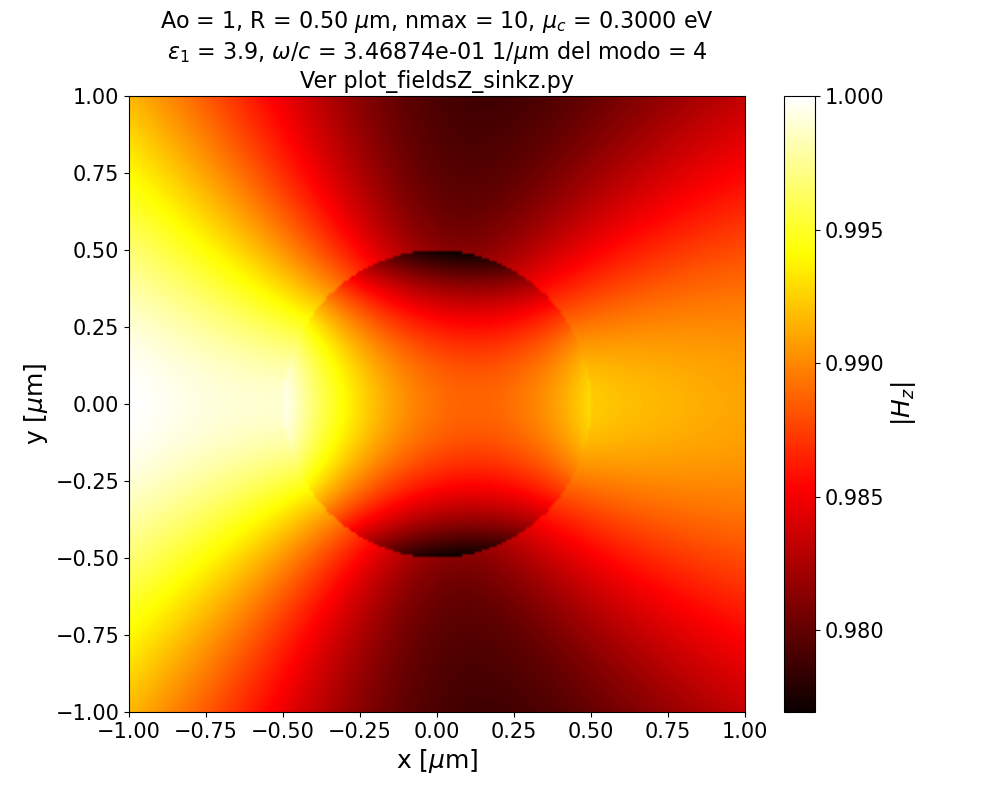
\includegraphics[width=0.2\textwidth]{results_non_disp/modHz_loss_modo4_mu0.3000.png}} 
    \caption{$|Hz|$ field with \fourNonDisp}
    \label{fig fields nondisp}
\end{figure}

In Fig \ref{fig fields nondisp}, for the active medium we used the critical values $[\Im\,\varepsilon_{1}]_c = -0.0353072, -0.0271857, -0.0282580, -0.0298547$ for the imaginary part of the permittivity of the active medium and $\omega_c/c =  [0.134005, 0.189642, 0.232135, 0.267846] $  $\mu m^{-1}$ for the dipolar, quadrupolar, hexapolar and octupolar modes.

%By comparing Fig.s \ref{fig fields nondisp}a and \ref{fig fields nondisp}b, obtained by evaluating the field distribution  at the resonant dipolar frequency, we observe that the field intensity is notably amplified ($\approx 10^{7}$) when the active medium takes a gain value close to the critical value $[\Im\,\varepsilon_{1}]_c$ for which the dipolar lasing threshold is achieved. For the other values of $[\Im\,\varepsilon_{1}]_c$ corresponding to the quadrupolar, hexapolar and octupolar modes we see that, besides amplification, the gain hides the interference between the scattered and the incident %fields  given place to a sharp field with well noticeable  modal characteristics. 
%field, thus producing sharp field distributions 
%which are a distinct signature of each amplified mode. 

By comparing the left and right columns of Fig.\ref{fig fields nondisp}, obtained by evaluating the field distribution at each resonant frequency, we observe important differences when the active medium takes a gain value close to the critical one, $[\Im\,\varepsilon_{1}]_c$.
These differences come from the interference with the incident plane wave. Basically, for gains far from the critical value, there is always interference between the fields produced by a given mode and the external source. However, close to the gain threshold, the fields produced by the eigenmodes are so strong that those coming from the external illumination become negligible.

%In Fig. \ref{fig fields nondisp} the enhancement of the fields given by adding an active medium inside the cylinder is illustrated. One advantage of the graphene-coated dielectric wire is that the field can penetrate into the interior regions, contrary to the metallic wires which are impenetrable and the fields are limited to a surface layer. 

%Thus the addition of an active medium using the critical value not only increase the intensity of the field in $10^8$ but also confines the field inside the cylinder. 

%As the Fig. \ref{fig fields nondisp} illustrates, the magnetic field $H_z$ follows the typical distribution for the dipolar, quadrupolar, hexapolar and octupolar patterns. Due to the presence of a surface current density $j_\varphi$ induced on the graphene sheet and the boundary conditions a discontinuity at $\rho = R$ is observed. 

\subsection{Dispersive medium}

We present rigorous numerical results obtained when the cylinder core is a 
%metallic-like 
metal-like material, with dielectric permittivity $\varepsilon_1(\omega)$ described by equation (\ref{eq permeabilidad 1 disp}). 
%which, in absence of gain, the dispersive characteristics are given by Eq. (\ref{eq drude lorentz}) 
We use $\varepsilon_\infty=3.9$, plasma frequency $\hbar \omega_p=0.6$eV and collision frequency $\hbar \gamma_{m}=0.01$eV. 
%As in the non-dispersive case, we found the numerical solutions of the equation \eqref{eq:disp01} by using the QE analytical expressions as initial guess. The is modeled by the equation \eqref{eq permeabilidad 1 disp}. 
%
\begin{figure}[h] %t
\centering
\includegraphics[width=0.49\textwidth]{results_disp/complex_poles1.png}
\caption{Complex poles (dipolar mode) for a cylinder with \oneDisp.} \label{fig complex poles disp}
\end{figure}
%

In Fig. \ref{fig complex poles disp} we show parametric curves in the 
complex frequency plane of the dipolar eigenfrequency calculated by solving the dispersion relation \eqref{eq:disp01}, as a parametric function of $\varepsilon_{di}$ for three different values of chemical potential $\mu_c = [0.3,0.6,0.9]$ eV. 
%$\Im\,\varepsilon_1$ for the dipolar mode and  
%
%\subsubsection{Complex poles}
%mismos comentarios que el caso no dispersivo
%
As in the non-dispersive case, a very small variation in the real part of the eigenfrequency is observed, 
%in each of the curves, 
which is consistent with the fact that the expression for the real part of the eigenfrequency predicted by the quasistatic approximation (\ref{eqn:QE dispersive2}) is independent of $\varepsilon_{di}$. 
However, the variation in the real part of the eigenfrequency is greater here than in the non-dispersive case (Figure \ref{fig complex poles non disp}), in agreement with the fact that 
obtaining \eqref{eqn:QE dispersive2} involves the use of approximations (in particular expanding in powers of $y=\frac{\varepsilon_{di}}{\varepsilon'_\infty+\varepsilon_2}$) that are not invoked to obtain  \eqref{eq:QE non dispersive2}. 
%
Moreover, we observe that the frequency region for the eigenfrequency trajectory is blue shifted when $\mu_{c}$ is increased from 0.3eV to 0.7eV. This is consistent with the fact that the hybridization formula (\ref{eqn:QE dispersive2}), obtained from the quasistatic  approximation, predicts a resonance frequency (real part of the eigenfrequency) which is proportional to $\sqrt{\omega_p^2+k\mu_c}$, $k=4 e^2/(\hbar^2 R)$.

%The QE approximation underestimate the losses thus the absolute value of the critical values in the numerical solution are bigger (not shown). 

%\subsubsection{Critical values}
%\label{sec critical values disp}

Fig. \ref{fig critical values disp} shows the critical values $[\varepsilon_{di}]_c $ for the first four modes as a function of chemical potential $\mu_c$ for two wires sizes: $R=0.5\mu$m (Fig. \ref{fig critical values disp}a) and $R=0.05\mu$m (Fig. \ref{fig critical values disp}b). 
%
Unlike the non dispersive case, where the active medium only has to compensate for plasmon losses in the graphene monolayer, in metal-like dispersive cores the active medium has to compensate for plasmon losses both in the graphene layer and in the nanocrystal. Thus, the modulus of the critical values $[\varepsilon_{di}]_c $ for all the graphene-nanocrystal hybridized plasmon modes shown in Fig. \ref{fig critical values disp} are bigger 
%($\approx 10$ times) 
than those for the graphene plasmons obtained in the non-dispersive case (Fig. \ref{fig critical values non disp}). 
\begin{figure}[ht!]
\centering
\captionsetup[subfigure]{justification=centering}
\subfloat[R = 0.5 $\mu$m]{\includegraphics[width=0.4\textwidth]{results_disp/im_epsi1_vs_muR_0.50.png}}
\newline
\captionsetup[subfigure]{justification=centering}
\subfloat[R = 0.05 $\mu$m]{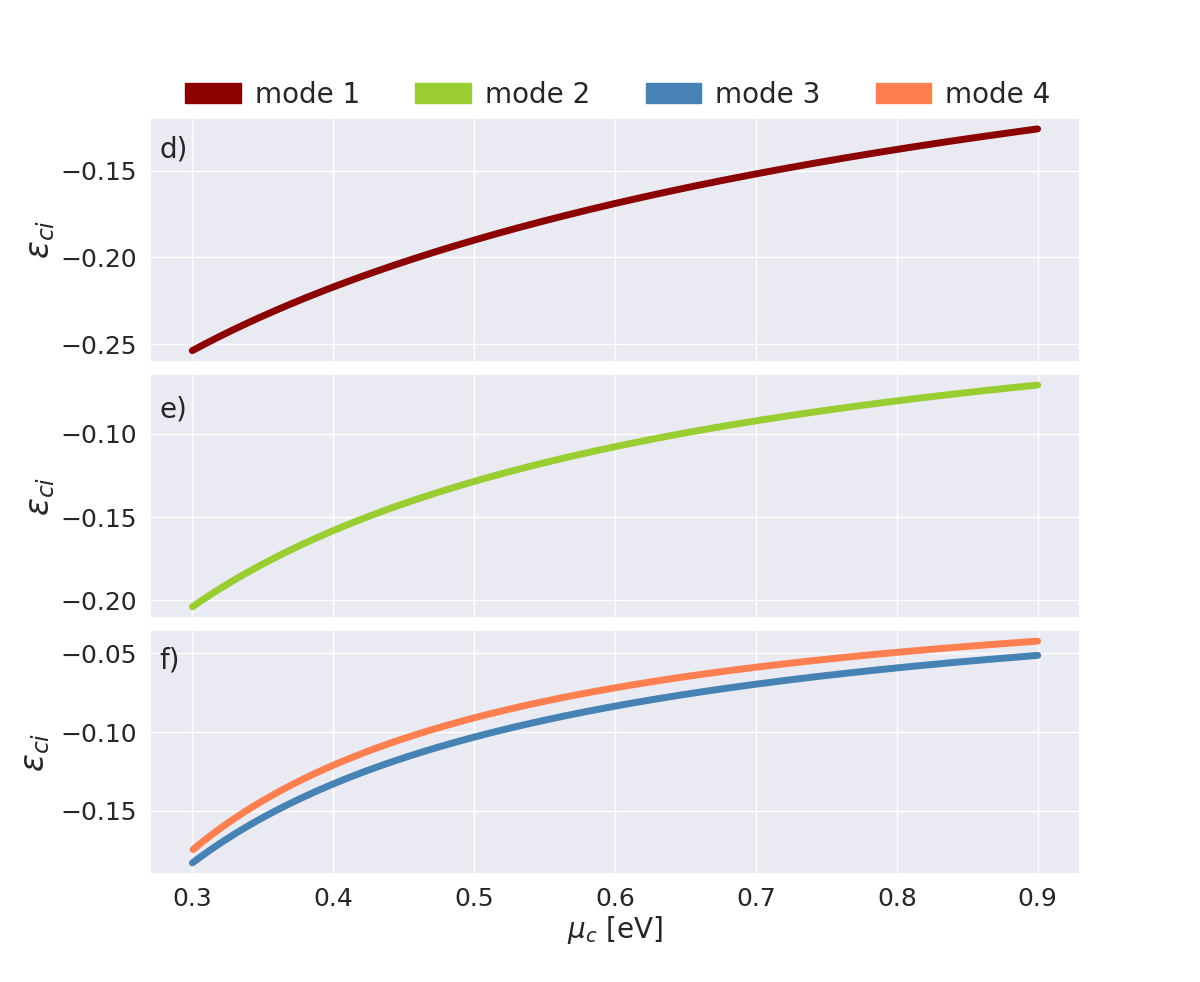
\includegraphics[width=0.4\textwidth]{results_disp/Im_epsi1_vs_muR_0.05.png}}
\caption{Critical values of $\varepsilon_{di}$ as a function of $\mu$ for for a cylinder with \twoDisp. 
%a) The dipolar mode. b) the quadrupolar mode c) The hexapolar and octupolar modes.
}
\label{fig critical values disp}
\end{figure}
%
%and this increment ($\approx 10$) is observed in all the modes (dipolar, quadrupolar, hexapolar and octupolar). 
%understanding  of  plasmonic losses  compensation  and  lasing  conditions
%Leila: ver  si esto es relevante, 
%That increment is a little higher in the dipolar mode ($\approx 3\cdot10$) which is consistent with the previous observation of the dipolar mode needing more optical gain. The better holding of the quasi-static approximation for higher modes is again observed. Nevertheless the QE approximation for the quadropolar mode non longer hold well. The dispersive behavior made more difficult the validation of the QE approximation thus it holds for higher modes than before (hexapolar and octupolar instead of quadrupolar, hexapolar and octupolar).   

Regarding wire size, Fig. \ref{fig critical values disp} clearly shows that the critical values corresponding to $R=0.05\mu$m (Fig. \ref{fig critical values disp}b) are notably lower than those corresponding to $R=0.5\mu$m (Fig. \ref{fig critical values disp}a). This reduction of the value of the critical gain with particle size 
%reduced with the decreasing of the particle size. This fact   %which does not occur in the metallic case without graphene, 
is anticipated by the quasistatic expression (\ref{eqn: frecuency crit QE dispersive}), which shows that  $|[\varepsilon_{di}]_c|$ is an increasing function of $R$ (note that the dependence on $R$ is included in $\omega^2_{0n}$). It is interesting to note that this behavior, which is absent in metallic cylinders without a graphene cover, results from the graphene-nanocristal plasmon hybridization and is highlighted when the effective plasma frequency $\omega_{on}$ is comparable with the nanocrystal plasma frequency $\omega_p$ (as is the case for the constitutive parameters chosen in this  example). 

%as follows. Taking into account that $\omega^2_{0n}\gamma_c<<\omega^2_{0n}$, the critical value $[\varepsilon_{di}]_c$ can be approached by 
%
%\begin{equation}
%\label{eqn: frecuency crit QE dispersive2}
%[\varepsilon_{di}]_c = - \dfrac{\omega^2_p \, %(\varepsilon'_\infty+\varepsilon_2)^{3/2}}{\Big(\omega^2_p+ \dfrac{4e^2}{\hbar^2\,R}\mu_c n %\Big)^{3/2}},
%\end{equation}
%
%where is straightforward to see 
%
%
%Leila: ver la relevancia de esto
%The Fig. \ref{fig critical values disp}a) illustrates the critical values of the dipolar mode and they have a  rectilinear shape thus the rectilinear movement of the charges inside a metallic-like medium (the medium inside the cylinder). 

%As in the non-dispersive case, when $\mu_c$ increas lo es the modulus of the critical value minimizes. However, that behavior for all the values of $\mu_c$ applied only for the higher modes in the first case and, as can be seen from Fig. \ref{fig critical values disp}a), the mentioned minimization occurred, for all the range of $\mu_c$, in the dipolar mode too. 

%The critical values depend on the metallic plasma frequency $\omega_p$. For higher value of $E_p$, the critical values increase in modulus (not show, \textcolor{red}{mostrarlo?}). The nanocrystal has more metallic behavior for bigger plasma frequency thus the metallic losses of the nanocrystal increases and the critical values needed are higher in modulus.  

%\subsubsection{Cross-sections}

%In Fig.s \ref{fig Qscat disp}, \ref{fig Qabs disp} and \ref{fig Qext disp} present the

In Fig. \ref{fig cross sections disp} we plot color maps, in the 
$\omega/c$ - $\Im\,\varepsilon_1$ plane, of the scattering (Fig. \ref{fig Qscat disp}), 
extinction (Fig. \ref{fig Qabs disp}) and absorption (Fig. \ref{fig Qext disp}) cross sections. 
%  and present the scattering,  absorption and  extinction cross sections, respectively. %Fig. \ref{fig cross sections disp} illustrates the improvement of the cross sections given by adding an active medium with critical value of Im($\varepsilon_1$). 
%\textcolor{gray}{As 
%it happened 
%in the non-dispersive 
%non dispersive se ha utilizado sin guión en muchas otras partes. También hay que decidir eso, para que sea todo igual. Siempre el guión es más correcto.
%case, the cross sections show an evident dipolar nature in this frequency range. Although we considered the first thirty modes in the field expansions(duda Ricardo).} 
We observe that the behavior around the critical point ($\omega_c/c$, $[\varepsilon_{di}]_c$)  is similar to that observed in the non-dispersive case (Fig. \ref{fig cross sections nondisp}), where the critical point falls on the full loss  compensation curve that separates the passive region (red region in Fig. \ref{fig Qext disp}) from the active region (blue region in Fig. \ref{fig Qext disp}).  

\begin{figure}[H]
    \centering
    \captionsetup[subfigure]{justification=centering}
    \subfloat[Scattering]{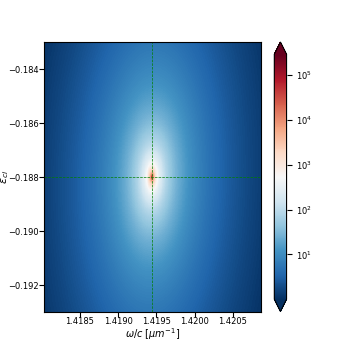
\includegraphics[width=0.22\textwidth]{results_disp/Qscat2D_modo1_mu0.3003_zoom.png}\label{fig Qscat disp}}
    \captionsetup[subfigure]{justification=centering}
    \subfloat[Absorption]{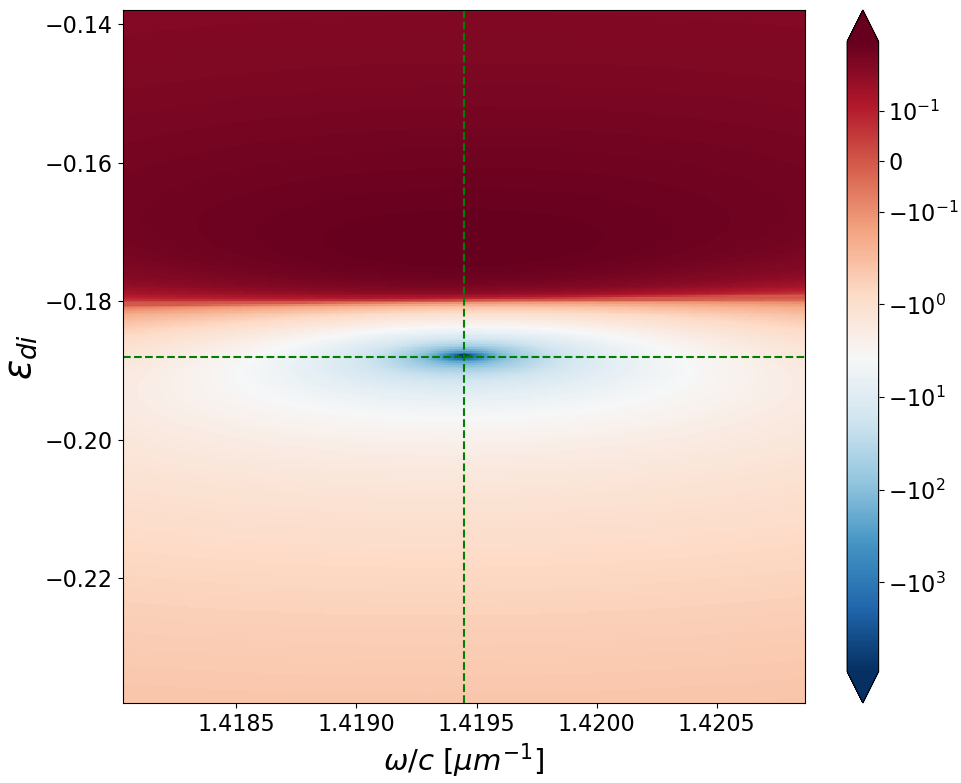
\includegraphics[width=0.22\textwidth]{results_disp/Qabs2D_modo1_mu0.3003_zoom.png}\label{fig Qabs disp}}
%    \newline
    \captionsetup[subfigure]{justification=centering}
    \subfloat[Extinction]{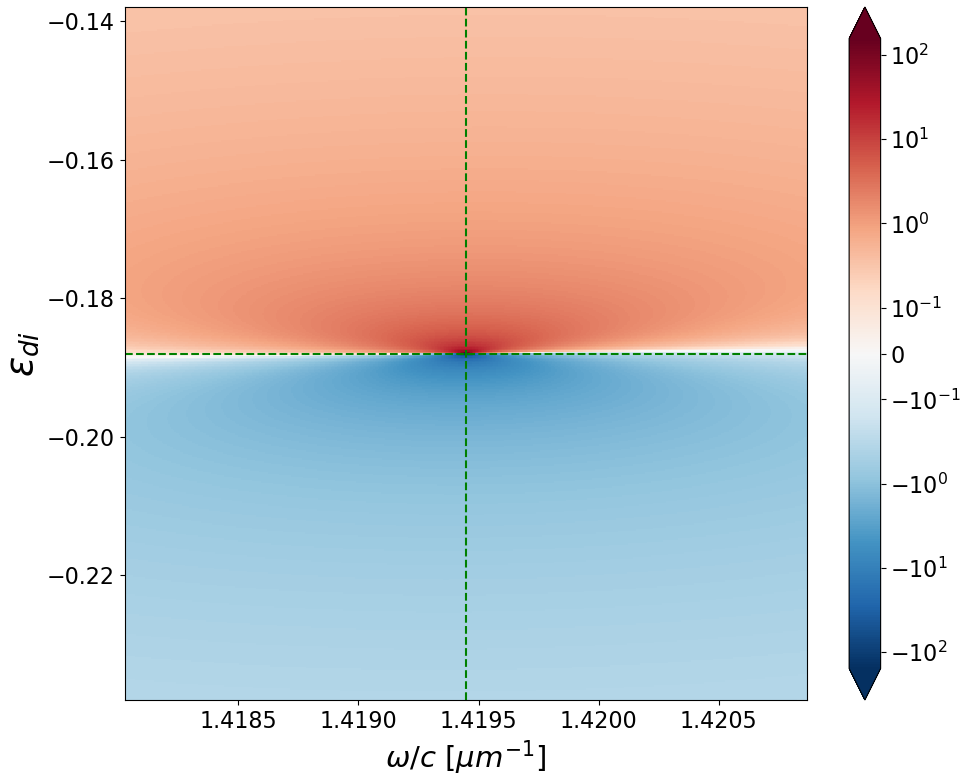
\includegraphics[width=0.22\textwidth]{results_disp/Qext2D_modo1_mu0.3003_zoom.png}\label{fig Qext disp}}
    \caption{Cross-section for a cylinder with \threeDisp. In green dotted lines: the critical values found before.}
    \label{fig cross sections disp}
\end{figure}

%Llegue hasta aca

%\subsubsection{Fields}

In Fig. \ref{fig fields disp} we  give color maps of the spatial distribution of the magnetic field 
%along the $\hat{z}$ direction 
for the first four modes. The right column corresponds to the case of a core without gain ($\varepsilon_{di}=0$), whereas the left column corresponds to the case of an active core  ($\varepsilon_{di} \neq 0$). 
The values of $\varepsilon_{di} \neq 0$ have been taken to obtain almost full loss  compensation for each mode. 
We used the critical values $[\varepsilon_{di}]_c = -0.253806, -0.203944, -0.183008, -0.174493$ for the imaginary part of the permittivity of the active medium and for the frequencies we used the values $\omega_c/c = [0.798031, 0.894243, 0.977434, 1.05174] $  $\mu m^{-1}$ for the dipolar, quadrupolar, hexapolar and octupolar modes. We again observe that the inclusion of gain inside the cylinder  sharply highlights  the multipolar characteristics of the near field. 
%
%We compared the $H_z$ field with active medium for different radius. 
%\begin{figure}[H]
%    \centering
%    \subfloat[R = 0.5 $\mu$m]{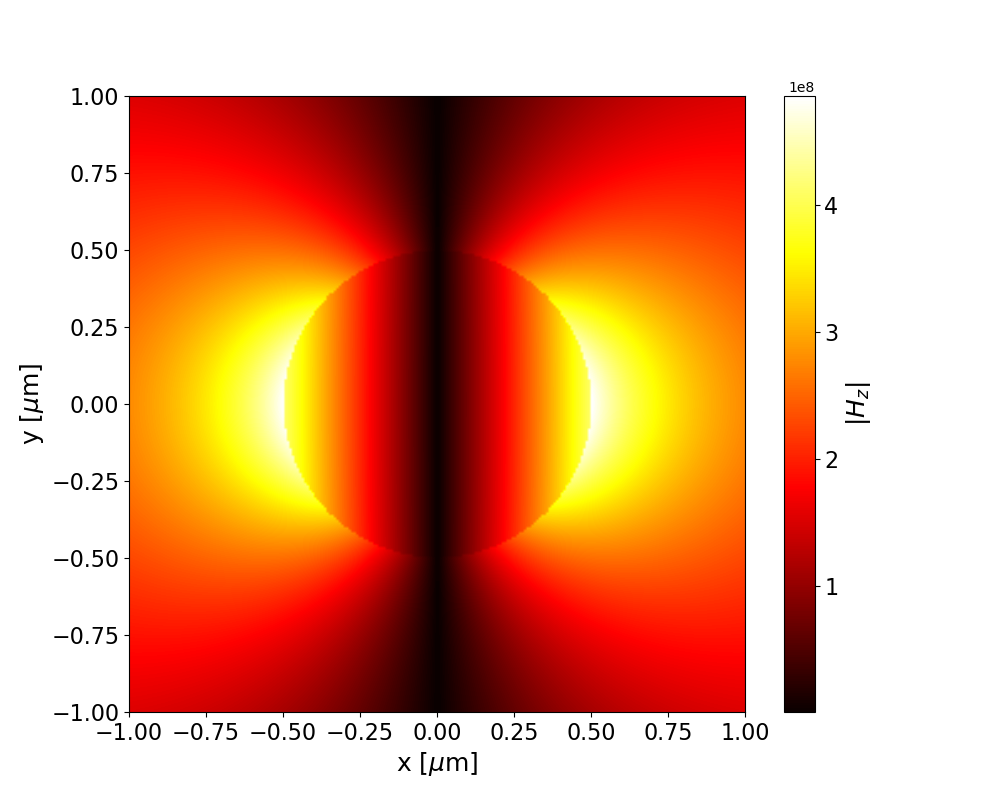
\includegraphics[width=0.2\textwidth]{results_disp/fields_vs_R/modHz_modo1_R0.500.png}}
%    \hspace{0.5mm}
%    \subfloat[R = 5.201 $\mu$m]{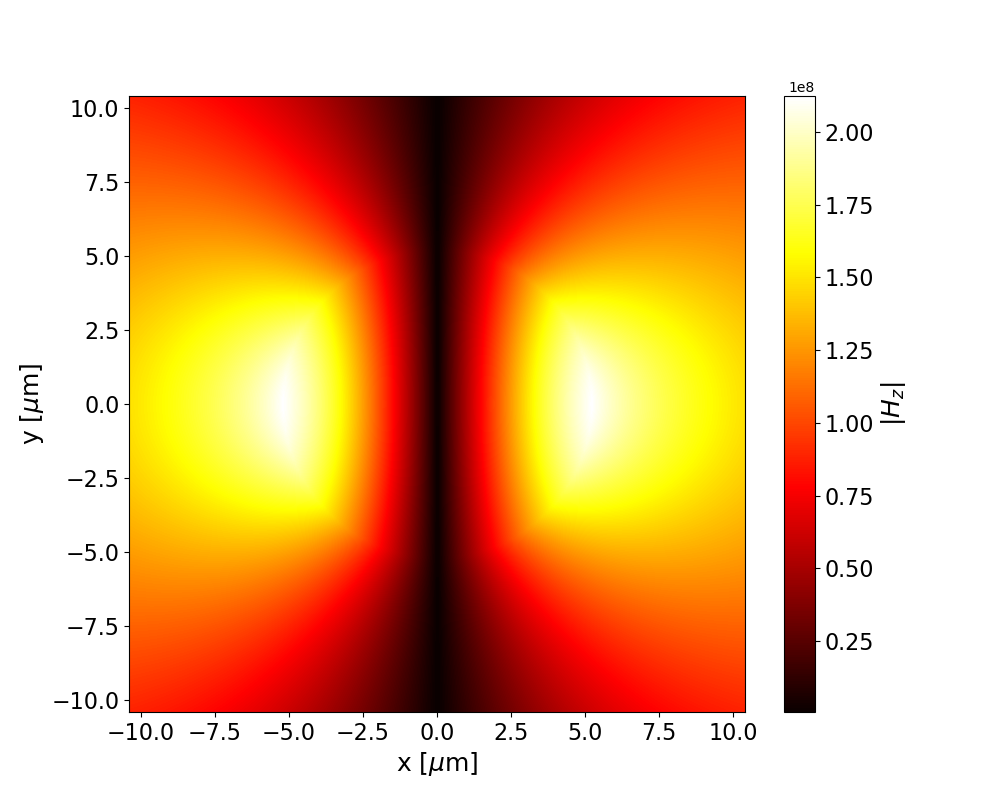
\includegraphics[width=0.2\textwidth]{results_disp/fields_vs_R/modHz_modo1_R5.201.png}} 
%    \newline
%    \subfloat[R = 0.5 $\mu$m]{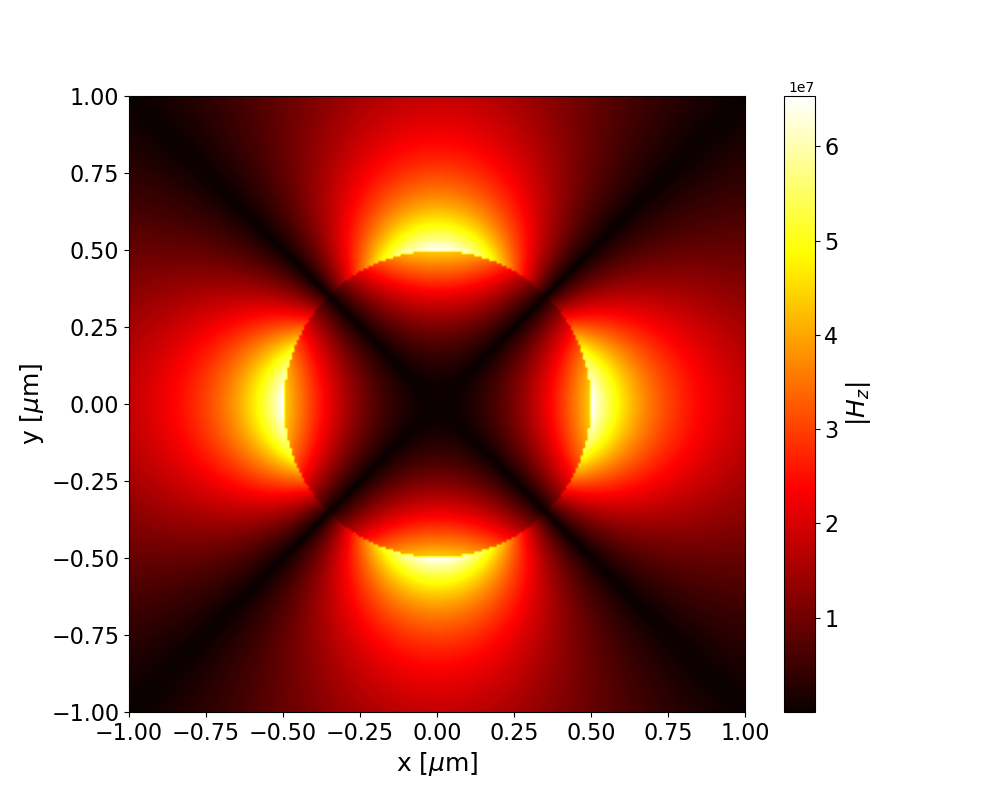
\includegraphics[width=0.2\textwidth]{results_disp/fields_vs_R/modHz_modo2_R0.500.png}}
%    \hspace{0.5mm}
%    \subfloat[R = 3.001 $\mu$m]{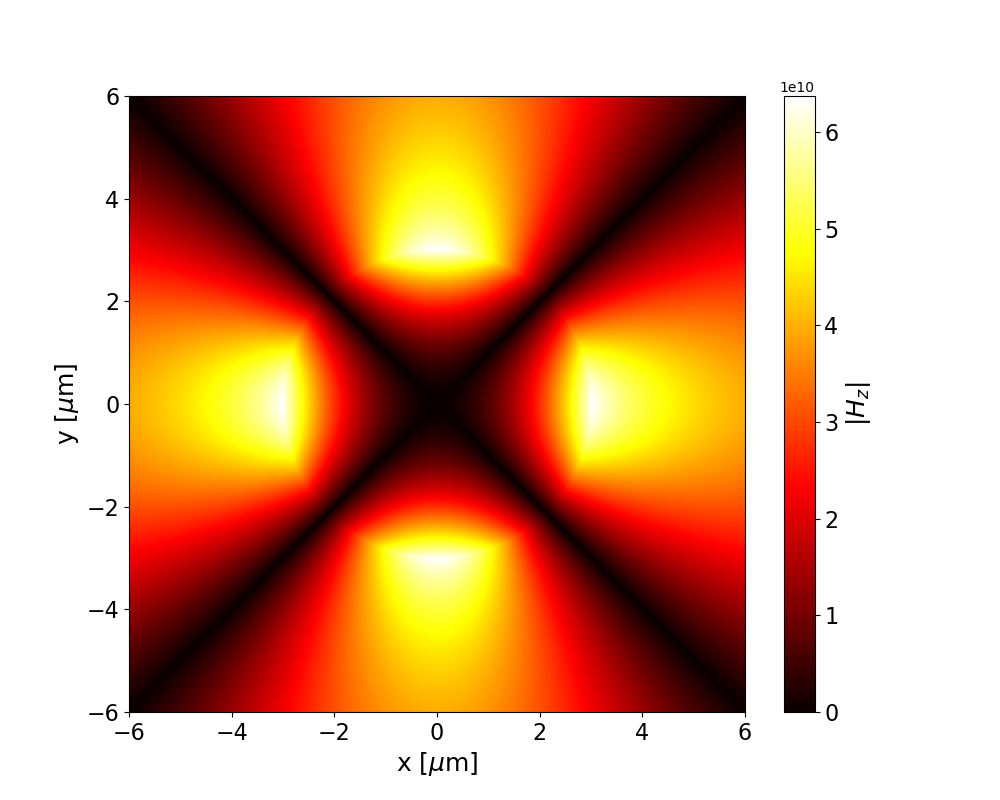
\includegraphics[width=0.2\textwidth]{results_disp/fields_vs_R/modHz_modo2_R3.001.png}} 
%    \caption{$|Hz|$ field with \fourDisp}
%    \label{fig fields disp radius}
%\end{figure}
%
%As can be seen from Fig. \ref{fig fields disp}d) (quadrupolar mode), for large core radii more field penetrates into the graphene cladding. For R = 3.361 $\mu$m, the plasmons resonate inside the cylinder and the modulus of the fields increases. The higher modes have better support with larger radius. 
%
%
%We observed an enhancement of the fields given by adding an active medium inside the cylinder and an increment of the intensity of the field in $10^8, 10^6,10^5,10^2$ for the first four modes, respectively. As the Fig. \ref{fig fields disp} show, the $H_z$ field distribution follows typical dipolar, quadrupolar, hexapolar and octupolar patterns. The field illustrates a symmetry under rotation because the angular dependence of the modes, given by exp(in$\varphi$), is the same for all the field components. 
%
%
%
\begin{figure}[ht!]
    \centering
    \captionsetup[subfigure]{justification=centering}
    \subfloat[mode 1, $\varepsilon_{di} \neq 0$]
    {\includegraphics[width=0.2\textwidth]{results_disp/fields_vs_mu/modHz_modo1_mu0.3000.png}}
    \hspace{1mm}
    \captionsetup[subfigure]{justification=centering}
    \subfloat[mode 1, $\varepsilon_{di} = 0$]
    {\includegraphics[width=0.2\textwidth]{results_disp/fields_vs_mu/modHz_loss_modo1_mu0.3000.png}} 
    \newline
    \captionsetup[subfigure]{justification=centering}
    \subfloat[mode 2, $\varepsilon_{di} \neq 0$]
    {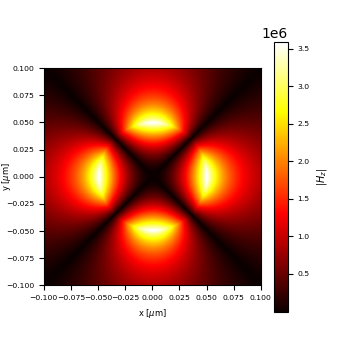
\includegraphics[width=0.2\textwidth]{results_disp/fields_vs_mu/modHz_modo2_mu0.3001.png}}
    \hspace{1mm}
    \captionsetup[subfigure]{justification=centering}
    \subfloat[mode 2, $\varepsilon_{di} = 0$]
    {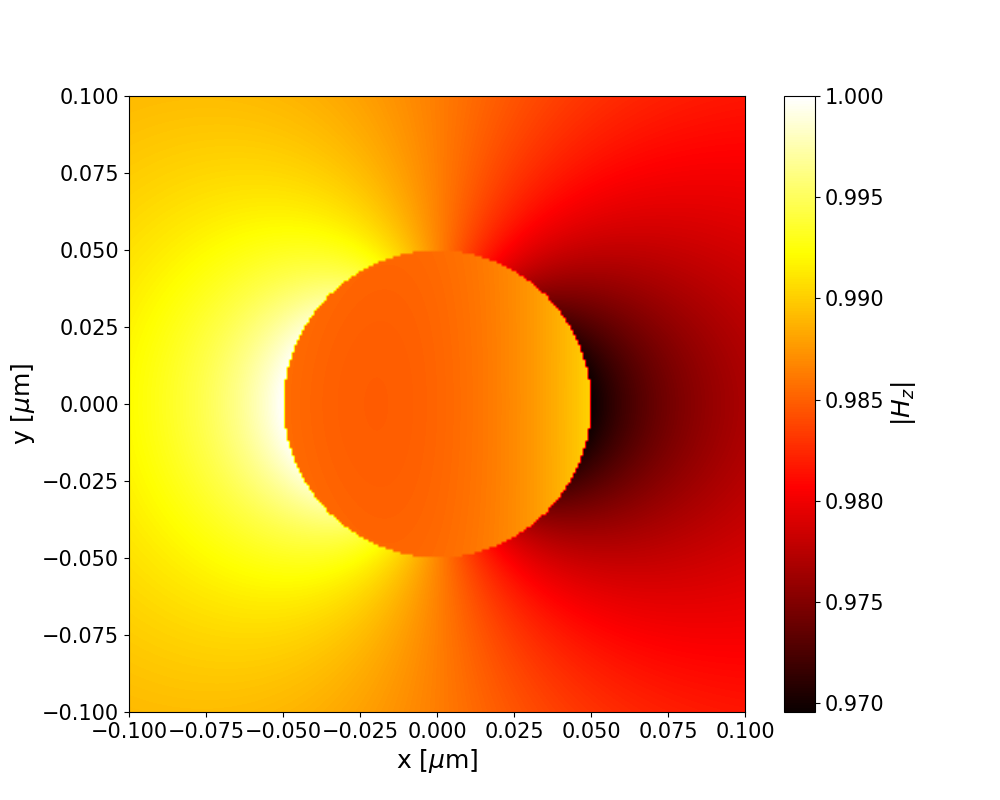
\includegraphics[width=0.2\textwidth]{results_disp/fields_vs_mu/modHz_loss_modo2_mu0.3001.png}} 
    \newline
    \captionsetup[subfigure]{justification=centering}
    \subfloat[mode 3, $\varepsilon_{di} \neq 0$]
    {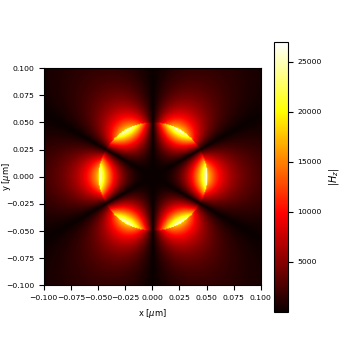
\includegraphics[width=0.2\textwidth]{results_disp/fields_vs_mu/modHz_modo3_mu0.3001.png}}
    \hspace{1mm}
    \captionsetup[subfigure]{justification=centering}
    \subfloat[mode 3, $\varepsilon_{di} = 0$]
    {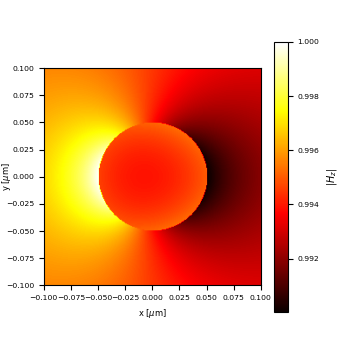
\includegraphics[width=0.2\textwidth]{results_disp/fields_vs_mu/modHz_loss_modo3_mu0.3001.png}} 
    \newline
    \captionsetup[subfigure]{justification=centering}
    \subfloat[mode 4, $\varepsilon_{di} \neq 0$]
    {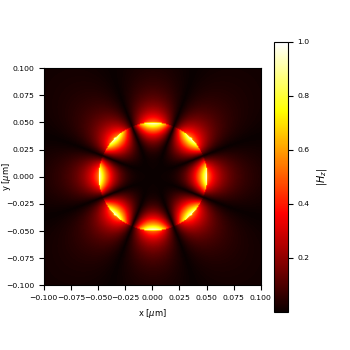
\includegraphics[width=0.2\textwidth]{results_disp/fields_vs_mu/modHz_modo4_mu0.3006.png}}
    \hspace{1mm}
    \captionsetup[subfigure]{justification=centering}
    \subfloat[mode 4, $\varepsilon_{di} = 0$]
    {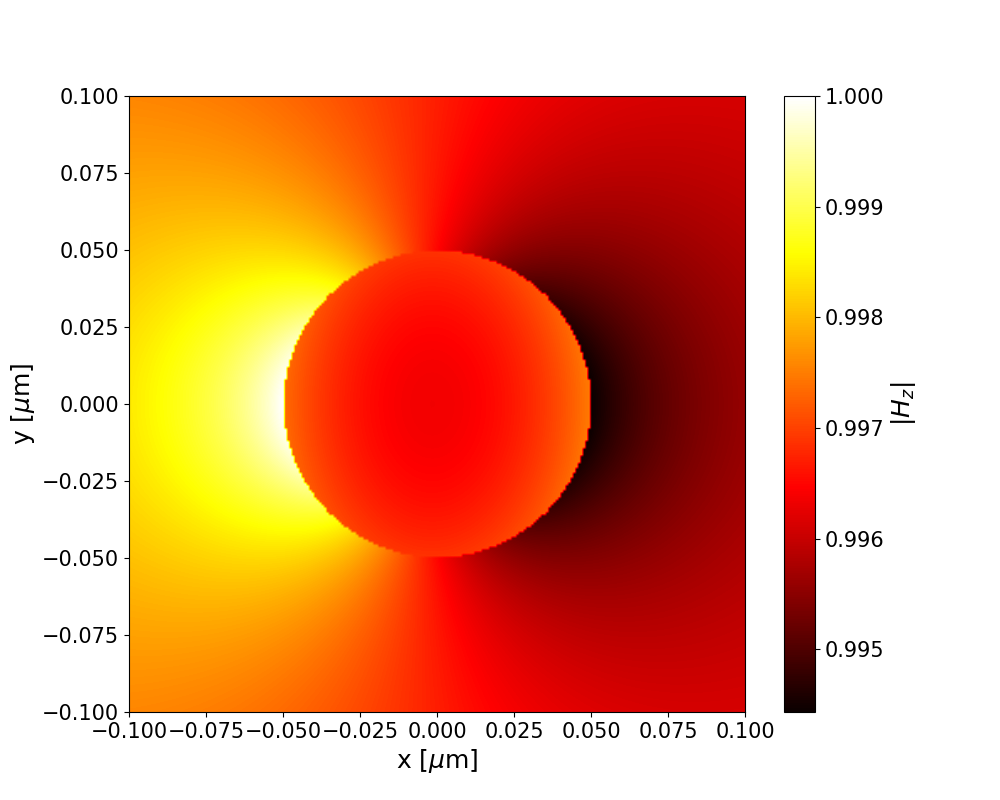
\includegraphics[width=0.2\textwidth]{results_disp/fields_vs_mu/modHz_loss_modo4_mu0.3006.png}} 
    \caption{$|Hz|$ field with \fourDisp}
    \label{fig fields disp}
\end{figure}

\section{Conclusion}

We have  investigated the lasing and optical amplification conditions for the LSP modes on a cylindrical wire wrapped with graphene. Regarding the material of the cylindrical wire, two different cases have been considered: an infrared/THz transparent material and a nanocrystal (a metal-like material). While in the first case the active medium compensates plasmon losses only in the graphene monolayer, in the second case the active medium compensates  losses both in the graphene layer and in the nanocrystal. 

In a first stage we  have used an eigenmode approach to calculate the trajectories of the eigenfrequencies in the complex frequency plane when the optical gain parameter is varied. 
This procedure allowed us to obtain the critical values of the optical gain for which a modal eigenfrequency trajectory crosses the real axis. It is for these critical values that the lasing condition is fulfilled for that mode. In a second stage, we have used an scattering approach which allowed us to get a complementary understanding of plasmonic 
losses compensation and lasing conditions in terms of scattering observables such as scattering, extinction and absorption cross sections. To analysis the results we invoke analytical expressions obtained by us using the quasistatic approximation. Our findings show that the studied systems present a wide frequency range tunability of lasing resonant states. Moreover, the gain modal critical values exhibit a great dependence on chemical potential. Wires with smaller radius show much  smaller gain modal critical values. Of the studied modes, the dipolar one showed the largest gain modal critical values. Both results suggest that radiative losses are the key factor controlling the gain modal critical values.


%Our results show that, besides the wide frequency range tunability of lasing resonant states, the gain modal critical values exhibit a great dependence on  chemical potential. We have observed that in these lasing states, and compared with a passive state, the absorption cross section of the graphene coated wire achieves a highly negative value, the scattering cross section is extraordinarily enhanced and the near field exhibits remarkable enhancements, whith sharp field distributions which are a distinct signature of each amplified mode. 


We believe that these results provide a deeper understanding of the characteristics of LSP spasers based on graphene and will motivate further exploration of other spaser configurations exploiting the optical advantages of the graphene electromagnetic response in the infrared and terahertz ranges. This may find numerous applications in terahertz spectroscopy, terahertz imaging, or in sensing of biological samples for example, where tissues are typically transparent to the frequency range studied.

\begin{backmatter}
\bmsection{Acknowledgments} 
We acknowledge financial support by Consejo Nacional de Investigaciones Cient\'ificas y T\'ecnicas (CONICET); Secretar\'ia de Ciencia y Tecnolog\'ia de la Universidad Nacional de C\'ordoba (SECYT-UNC); and Agencia Nacional de Promoci\'on Cient\'ifica y Tecnol\'ogica (ANPCyT, PICT-2018-03587).
\bmsection{Disclosures}
The authors declare no conflicts of interest.
\end{backmatter}


%\appendix
%\section{Appendixes}


%Sets the bibliography style to UNSRT and imports the 
%bibliography file "samples.bib".
%\bibliographystyle{phys}

\medskip %importante para el espaciamiento, no sacar
\bibliography{PrelatCilGraf01}
%\printbibliography
% Produces the bibliography via BibTeX.


\end{document}
%
% ****** End of file apssamp.tex ******

